\section{Risultati}
\newcommand{\epsmx}{$\varepsilon_{max}$}
La validazione dei modelli appena discussi è stata effettuata confrontando i
risultati della simulazione con le stime dedotte dall'analisi, valutando quattro
possibili scenari contraddistinti dal valore che assume il parametro $S$.

Ognuno di questi scenari è stato simulato facendo processare al programma lo
stesso numero di job affinché le statistiche globali del sistema possano
essere confrontate. Tale numero è stato stabilito in base alle metriche che
andavano valutate ed al numero di job che le riguardava.

Lo scenario con valore di soglia $S=5$, è quello in cui soltanto circa il $2\%$
dei job di classe 2 è processato nel cloudlet e di questi circa il $90\%$
vengono interrotti, ne risulta, quindi che in relazione al numero totale dei job
che transitano nel sistema, solamente lo $0.14\%$ sono job di classe 2
processati con successo nel cloudlet e l'$1.37\%$ sono job interrotti. In
definitiva, al fine di avere una dimensione dei batch soddisfacente per il
calcolo delle relative metriche, è stato scelto un numero totale di job pari a
$500000$. In questo modo si ottiene un numero di job di classe 2 processati con
successo nel cloudlet pari a circa $700$ e un numero di job interrotti pari a
circa $6850$, ciò significa che per un valore $k=64$ corrispondente al numero
di batch, si ottengono batch di dimensione $10$ e $107$ rispettivamente, che
sono sufficienti a determinare intervalli di confidenza, seppur con un ampio
margine di errore.

Quello appena descritto è il peggior scenario possibile, in cui si registra il
minor numero di job per una determinata metrica, gli altri scenari vengono
quindi simulati tutti con un numero totale di job pari a $500000$, e a seconda
del numero di job che verranno processati nei vari nodi e della loro tipologia,
sono risultati intervalli di confidenza più o meno precisi.

Purtroppo è risultato impossibile determinare risultati attendibili per i job
di classe 1 che vengono processati nel cloud, poiché il loro numero è, per ogni
scenario, talmente esiguo, che per avere un batch di dimensione 10 sarebbero
necessari almeno 3 milioni di job in tutto. Tuttavia, con un numero di
$500000$ job totali, si ottengono delle statistiche globali molto attendibili,
infatti, ad esempio per il tempo medio di risposta del sistema, si ottiene 
una dimensione del batch pari a $\lfloor\frac{500000}{64}\rfloor = 7812$.

Per ogni statistica vengono presentati grafici e tabelle, in cui vengono
confrontati i risulatati osservati in 10 repliche della simulazione con la
relativa stima del modello analitico, inoltre nelle tabelle viene anche indicato
l'errore massimo che è stato commesso, corrispondente al massimo delle distanze 
tra la stima e l'estremo più lontano di ogni intervallo di confidenza.
%
%
%%%%%%%%%%%%%%%%%%%%%%%%%%%%%%%%%%%%%%%%%%%%%%%%%%%%%%%%%%%%%%%%%%%%%%%%%%%%%%%%
%%%%%%%%%%%%%%%%%%%%%%%%%%%%%%%%%%%%%%%%%%%%%%%%%%%%%%%%%%%%%%%%%%%%%%%%%%%%%%%%
%%%%%%%%%%%%%%%%%%%%%%%%%%%%%%%%%%%%%%%%%%%%%%%%%%%%%%%%%%%%%%%%%%%%%%%%%%%%%%%%
\subsection{Percentuale Interruzioni}
Per comprendere al meglio l'analisi delle simulazioni ed il confronto con le
stime effettuate è conveniente iniziare dalla presentazione dei risultati
riguardanti la percentuale di job di classe 2 interrotti, poiché da questi
dipendono la maggior parte delle metriche successive.

I grafici in figura~\ref{plot:intperc} mostrano che, nei casi in cui
$S=20,15,10$, la stima della percentuale di interruzione risulta leggermente
inferiore dei valori osservati nelle simulazioni e l'errore massimo che viene
commesso è di circa il $5$-$6\%$, mentre per quanto riguarda il caso in cui
$S=5$ si ottiene una stima leggermente migliore, ma ciò è dovuto al basso
valore della soglia che impedisce ai job di classe 2 di accedere al cloudlet, di
conseguenza è stata riscontrata una maggiore variabilità dei valori delle
simulazioni e si commette infatti un'errore massimo più alto pari al $7.6\%$.

La maggiore percentuale di job interrotti (circa del $30\%$ considerando le
varie repliche), si ottiene per $S=10$, mentre nei restanti due casi non si
hanno valori troppo discordanti, differiscono infatti di circa un punto
percentuale.

I valori delle simulazioni e gli errori relativi rispetto alla stima del modello
analitico sono riportati nelle
tabella~\ref{tab:intperc}.
%
\begin{figure}[!h]
\centering
%
\begin{subfigure}[t]{0.49\textwidth}
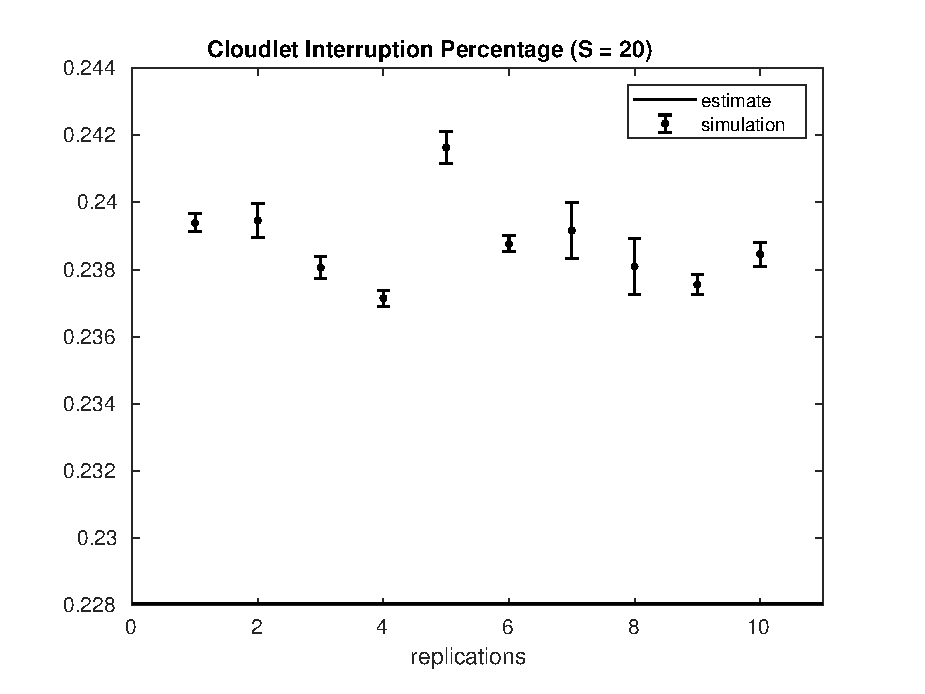
\includegraphics[width=\textwidth]{figures/simul/20_500K_intperc}
\caption{$S = 20$}
\label{20_intperc}
\end{subfigure}
%
\begin{subfigure}[t]{0.49\textwidth}
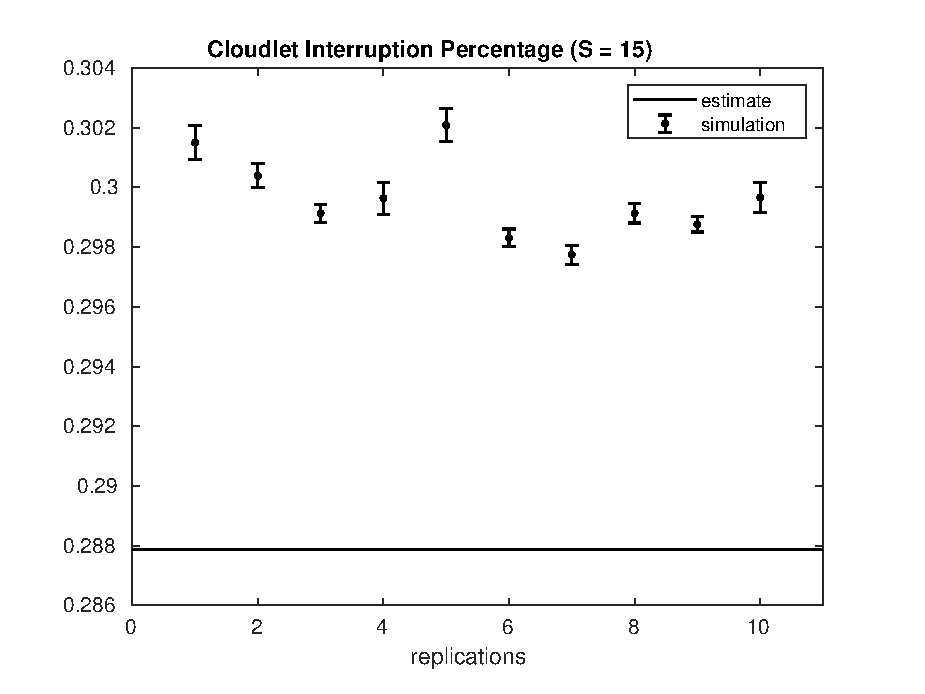
\includegraphics[width=\textwidth]{figures/simul/15_500K_intperc}
\caption{$S = 15$}
\label{15_intperc}
\end{subfigure}
%
\begin{subfigure}[t]{0.49\textwidth}
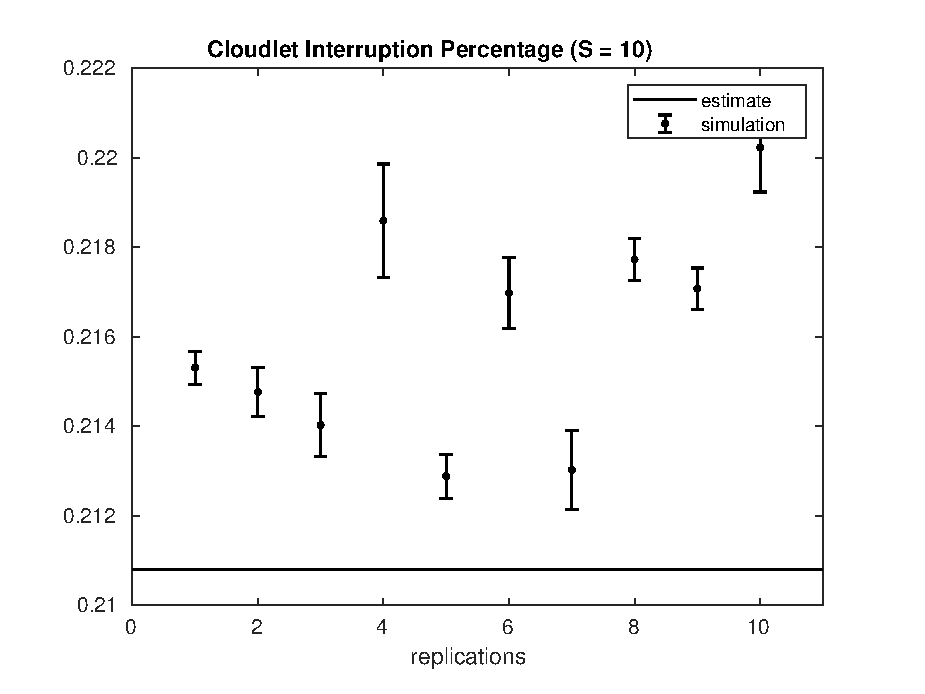
\includegraphics[width=\textwidth]{figures/simul/10_500K_intperc}
\caption{$S = 10$}
\label{10_intperc}
\end{subfigure}
%
\begin{subfigure}[t]{0.49\textwidth}
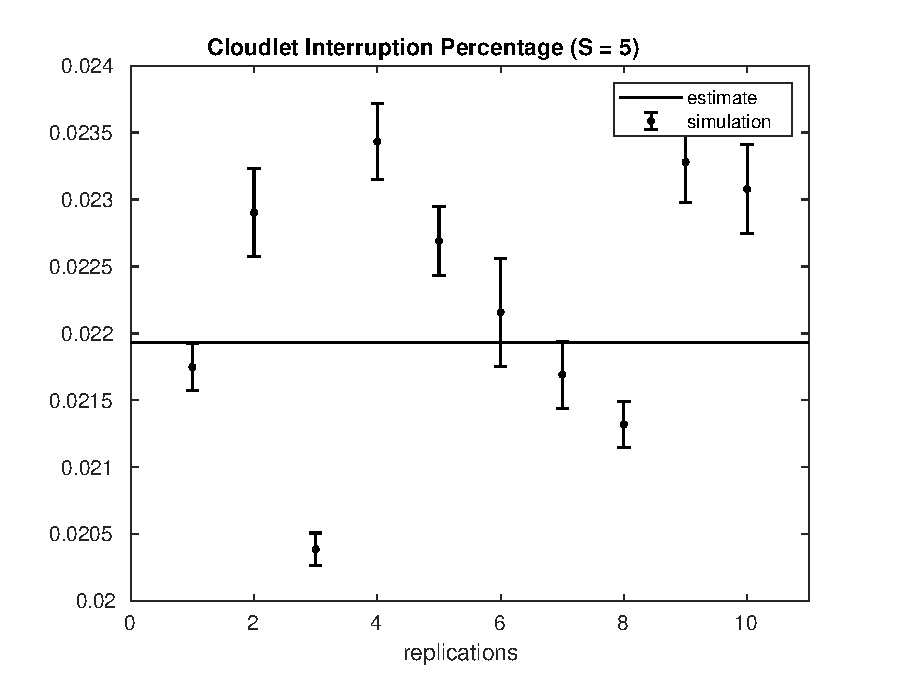
\includegraphics[width=\textwidth]{figures/simul/5_500K_intperc}
\caption{$S = 5$}
\label{5_intperc}
\end{subfigure}
%
\caption{Percentuale di interruzioni}
\label{plot:intperc}
\end{figure}
%
%
\begin{table}[!h]
\begin{adjustbox}{width=\textwidth}
\begin{tabular}{c|r@{.}l|r@{.}l|r@{.}l|r@{.}l}
& \multicolumn{2}{|c|}{$S=20$}
& \multicolumn{2}{|c}{$S=15$}
& \multicolumn{2}{|c}{$S=10$}
& \multicolumn{2}{|c}{$S=5$}
\\          
\hline
R1     & $0$&$2394 \pm 0.0003$ & $0$&$3015 \pm 0.0006$ & $0$&$2153 \pm 0.0004$ & $0$&$0217 \pm 0.0002$ \\
R2     & $0$&$2395 \pm 0.0005$ & $0$&$3004 \pm 0.0004$ & $0$&$2148 \pm 0.0005$ & $0$&$0229 \pm 0.0003$ \\
R3     & $0$&$2381 \pm 0.0003$ & $0$&$2991 \pm 0.0003$ & $0$&$2140 \pm 0.0007$ & $0$&$0204 \pm 0.0001$ \\
R4     & $0$&$2371 \pm 0.0002$ & $0$&$2996 \pm 0.0005$ & $0$&$2186 \pm 0.0013$ & $0$&$0234 \pm 0.0003$ \\
R5     & $0$&$2416 \pm 0.0005$ & $0$&$3021 \pm 0.0006$ & $0$&$2129 \pm 0.0005$ & $0$&$0227 \pm 0.0003$ \\
R6     & $0$&$2388 \pm 0.0002$ & $0$&$2983 \pm 0.0003$ & $0$&$2170 \pm 0.0008$ & $0$&$0222 \pm 0.0004$ \\
R7     & $0$&$2392 \pm 0.0008$ & $0$&$2977 \pm 0.0003$ & $0$&$2130 \pm 0.0009$ & $0$&$0217 \pm 0.0003$ \\
R8     & $0$&$2381 \pm 0.0008$ & $0$&$2991 \pm 0.0003$ & $0$&$2177 \pm 0.0005$ & $0$&$0213 \pm 0.0002$ \\
R9     & $0$&$2376 \pm 0.0003$ & $0$&$2988 \pm 0.0003$ & $0$&$2171 \pm 0.0005$ & $0$&$0233 \pm 0.0003$ \\
R10    & $0$&$2385 \pm 0.0004$ & $0$&$2997 \pm 0.0005$ & $0$&$2202 \pm 0.0010$ & $0$&$0231 \pm 0.0003$ \\
EST    & $0$&$2280$            & $0$&$2879$            & $0$&$2108$            & $0$&$0219$            \\
\epsmx & $0$&$0141 \ (5.8\%)$  & $0$&$0148 \ (4.9\%)$  & $0$&$0104 \ (4.7\%)$  & $0$&$0018 \ (7.6\%)$    
\end{tabular}
\end{adjustbox}
\caption{percentuale job di classe 2 interrotti $S=20$}
\label{tab:intperc}
\end{table}

%%%%%%%%%%%%%%%%%%%%%%%%%%%%%%%%%%%%%%%%%%%%%%%%%%%%%%%%%%%%%%%%%%%%%%%%%%%%%%%%
\subsection{Tempo di Risposta Cloudlet Classe 1}
Il tempo di risposta per un job di classe 1 che viene eseguito nel cloudlet è
indipendente dal parametro S ed i risultati presentati in
figura~\ref{plot:s1clet} e nella tabella~\ref{tab:s1clet} mostrano che tutti gli
intervalli di confidenza calcolati comprendono il valore stimato ed il valore
dell'errore massimo è sotto la soglia dell'$1\%$ in ogni caso.
\begin{figure}[!h]
\centering
%
\begin{subfigure}[t]{0.49\textwidth}
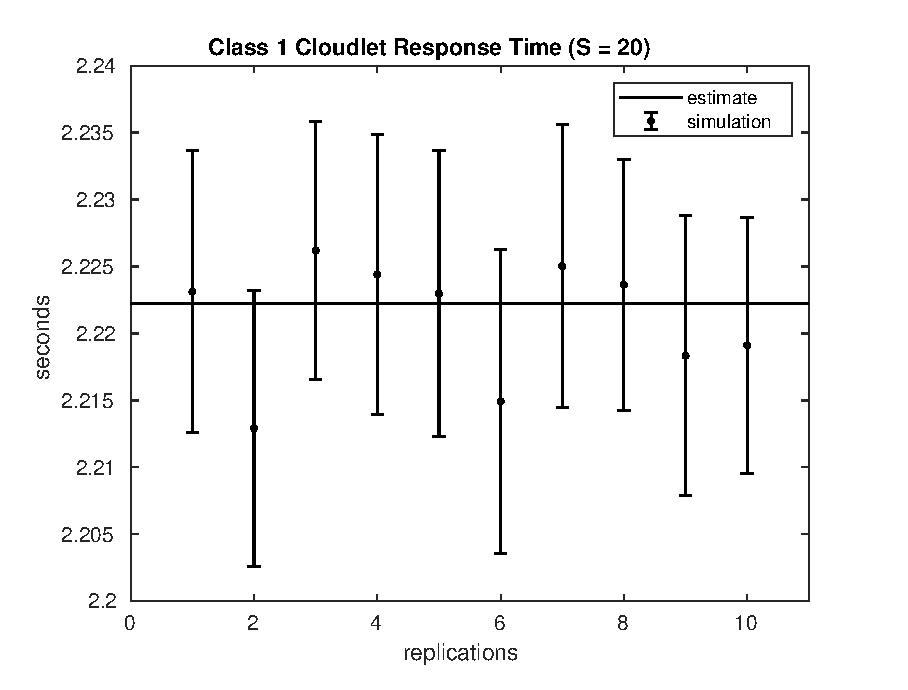
\includegraphics[width=\textwidth]{figures/simul/20_500K_s1clet}
\caption{$S = 20$}
\label{20_s1clet}
\end{subfigure}
%
\begin{subfigure}[t]{0.49\textwidth}
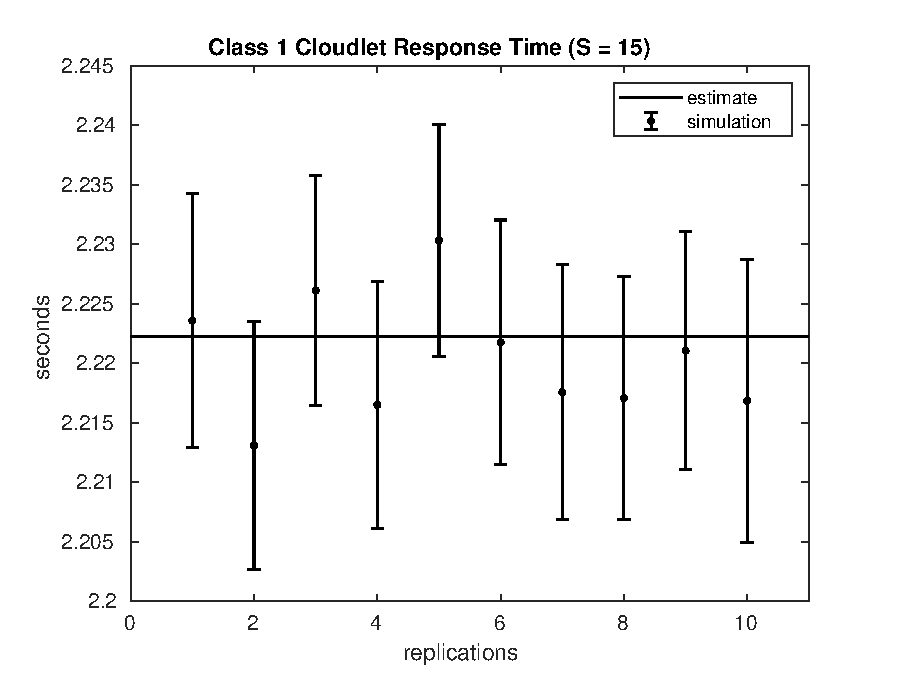
\includegraphics[width=\textwidth]{figures/simul/15_500K_s1clet}
\caption{$S = 15$}
\label{15_s1clet}
\end{subfigure}
%
\begin{subfigure}[t]{0.49\textwidth}
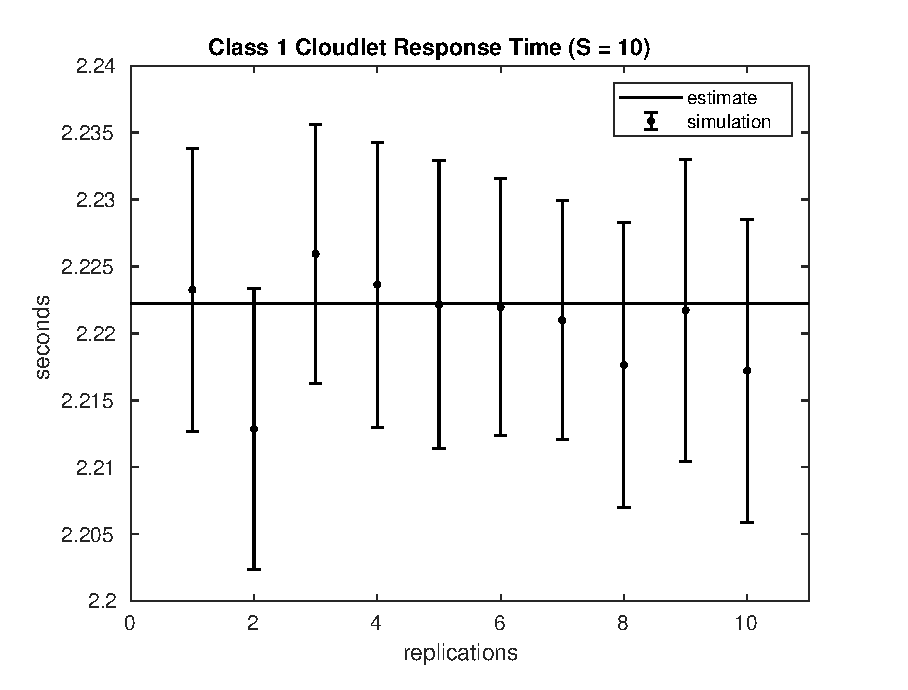
\includegraphics[width=\textwidth]{figures/simul/10_500K_s1clet}
\caption{$S = 10$}
\label{10_s1clet}
\end{subfigure}
%
\begin{subfigure}[t]{0.49\textwidth}
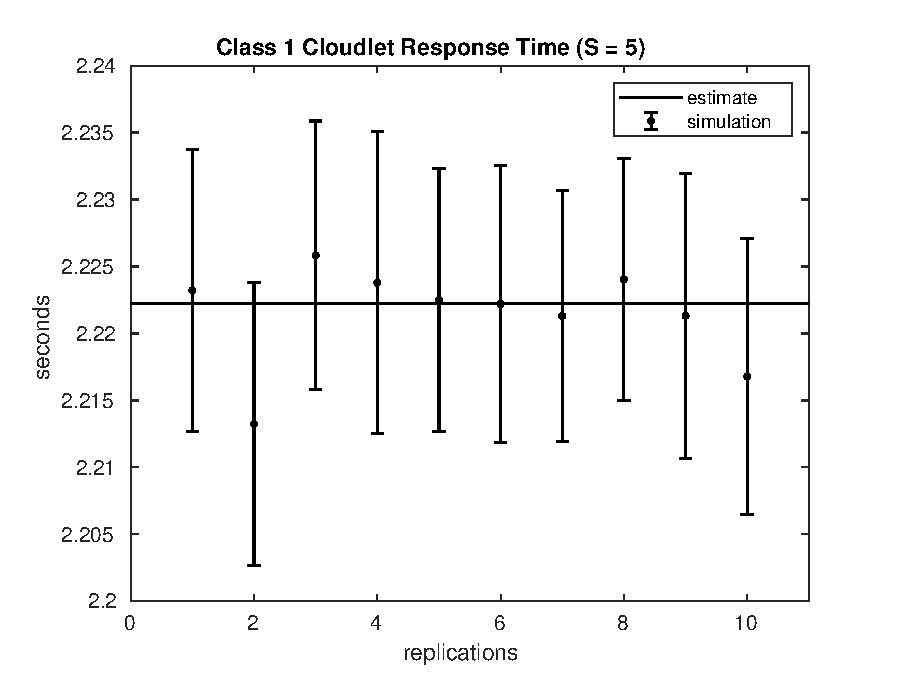
\includegraphics[width=\textwidth]{figures/simul/5_500K_s1clet}
\caption{$S = 5$}
\label{5_s1clet}
\end{subfigure}
%
\caption{tempo di risposta cloudlet classe 1}
\label{plot:s1clet}
\end{figure}
%
%
\begin{table}[!h]
\begin{adjustbox}{width=\textwidth}
\begin{tabular}{c|r@{.}l|r@{.}l|r@{.}l|r@{.}l}
& \multicolumn{2}{|c|}{$S=20$}
& \multicolumn{2}{|c|}{$S=15$}
& \multicolumn{2}{|c|}{$S=10$}
& \multicolumn{2}{|c}{$S=5$}
\\          
\hline
R1      & $2$&$2231 \pm 0.0105$ & $2$&$2236 \pm 0.0107$ & $2$&$2233 \pm 0.0106$ & $2$&$2231 \pm 0.0105$ \\
R2      & $2$&$2129 \pm 0.0103$ & $2$&$2131 \pm 0.0104$ & $2$&$2129 \pm 0.0105$ & $2$&$2129 \pm 0.0103$ \\
R3      & $2$&$2262 \pm 0.0096$ & $2$&$2261 \pm 0.0096$ & $2$&$2259 \pm 0.0097$ & $2$&$2262 \pm 0.0096$ \\
R4      & $2$&$2244 \pm 0.0105$ & $2$&$2165 \pm 0.0104$ & $2$&$2236 \pm 0.0106$ & $2$&$2244 \pm 0.0105$ \\
R5      & $2$&$2230 \pm 0.0107$ & $2$&$2303 \pm 0.0097$ & $2$&$2222 \pm 0.0107$ & $2$&$2230 \pm 0.0107$ \\
R6      & $2$&$2149 \pm 0.0113$ & $2$&$2218 \pm 0.0103$ & $2$&$2220 \pm 0.0096$ & $2$&$2149 \pm 0.0113$ \\
R7      & $2$&$2250 \pm 0.0106$ & $2$&$2176 \pm 0.0107$ & $2$&$2210 \pm 0.0089$ & $2$&$2250 \pm 0.0106$ \\
R8      & $2$&$2236 \pm 0.0094$ & $2$&$2171 \pm 0.0102$ & $2$&$2177 \pm 0.0107$ & $2$&$2236 \pm 0.0094$ \\
R9      & $2$&$2183 \pm 0.0104$ & $2$&$2211 \pm 0.0100$ & $2$&$2217 \pm 0.0113$ & $2$&$2183 \pm 0.0104$ \\
R10     & $2$&$2191 \pm 0.0095$ & $2$&$2168 \pm 0.0119$ & $2$&$2172 \pm 0.0113$ & $2$&$2191 \pm 0.0095$ \\
EST     & $2$&$2222$            & $2$&$2222$            & $2$&$2222$            & $2$&$2222$            \\
\epsmx  & $0$&$0136 \ (0.6\%)$  & $0$&$0178 \ (0.8\%)$  & $0$&$0134 \ (0.6\%)$  & $0$&$0136 \ (0.6\%)$    
\end{tabular}
\end{adjustbox}
\caption{tempo di risposta cloudlet classe 1}
\label{tab:s1clet}
\end{table}

%%%%%%%%%%%%%%%%%%%%%%%%%%%%%%%%%%%%%%%%%%%%%%%%%%%%%%%%%%%%%%%%%%%%%%%%%%%%%%%%
\subsection{Tempo di Risposta Cloudlet Classe 2}
La figura~\ref{plot:s2clet} e la tabella~\ref{tab:s2clet} mostrano un tempo di
risposta medio per i job di classe 2 eseguiti nel cloudlet che cresce/decresce
in modo proporzionale ad $S$, ciò sta a indicare che la probabilità di
interruzione di un job in esecuzione nel cloudlet ($P_{intr}^{clet}$) è
inversamente proporzionale a $S$ ed incide maggiormente nell'abbattimento del
tempo di risposta laddove $S$ è minore.

La stima effettuata, nei casi in cui $S=20,15,10$, è affidabile con un errore
massimo del $5\%$, mentre, nel caso in cui $S=5$, gli intervalli di confidenza
hanno un ampiezza eccessiva con un errore anche del $104\%$, quest'ultimo fatto
è dovuto al basso valore del parametro di soglia e all'elevato tasso di
interruzione per i job accettati nel nodo, risulta così un ridotto numero di job
di classe 2 che vengono processati nel cloudlet, e di conseguenza una dimensione
dei batch troppo piccola per ottenere intervalli precisi.
\begin{figure}[!h]
\centering
%
\begin{subfigure}[t]{0.49\textwidth}
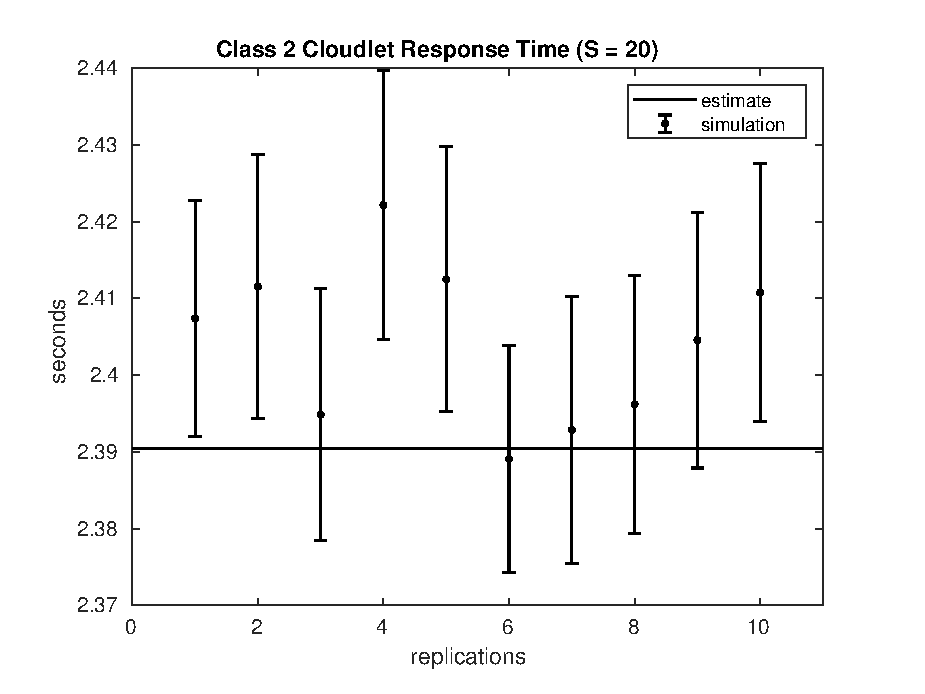
\includegraphics[width=\textwidth]{figures/simul/20_500K_s2clet}
\caption{$S = 20$}
\label{20_s2clet}
\end{subfigure}
%
\begin{subfigure}[t]{0.49\textwidth}
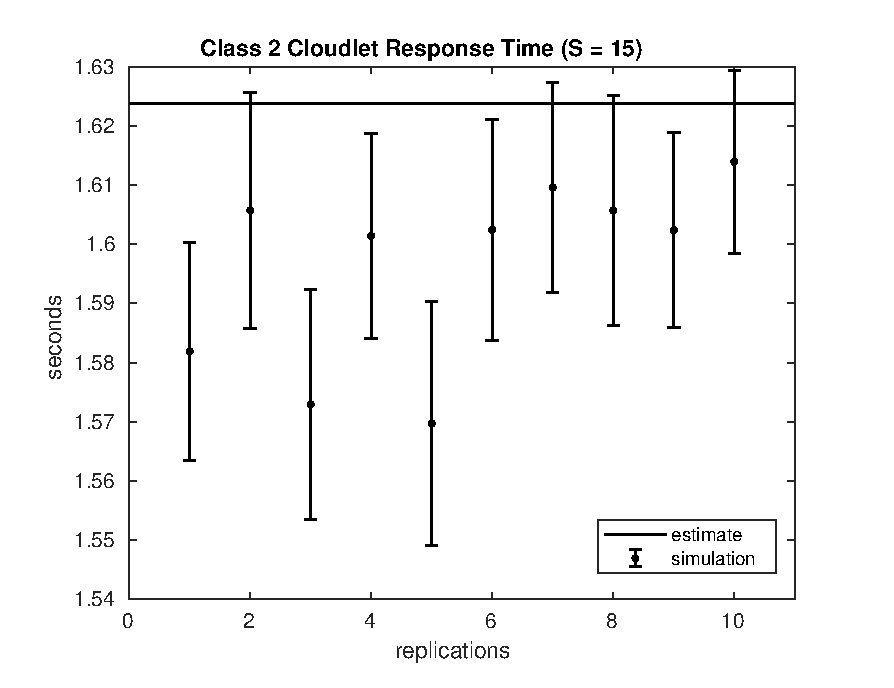
\includegraphics[width=\textwidth]{figures/simul/15_500K_s2clet}
\caption{$S = 15$}
\label{15_s2clet}
\end{subfigure}
%
\begin{subfigure}[t]{0.49\textwidth}
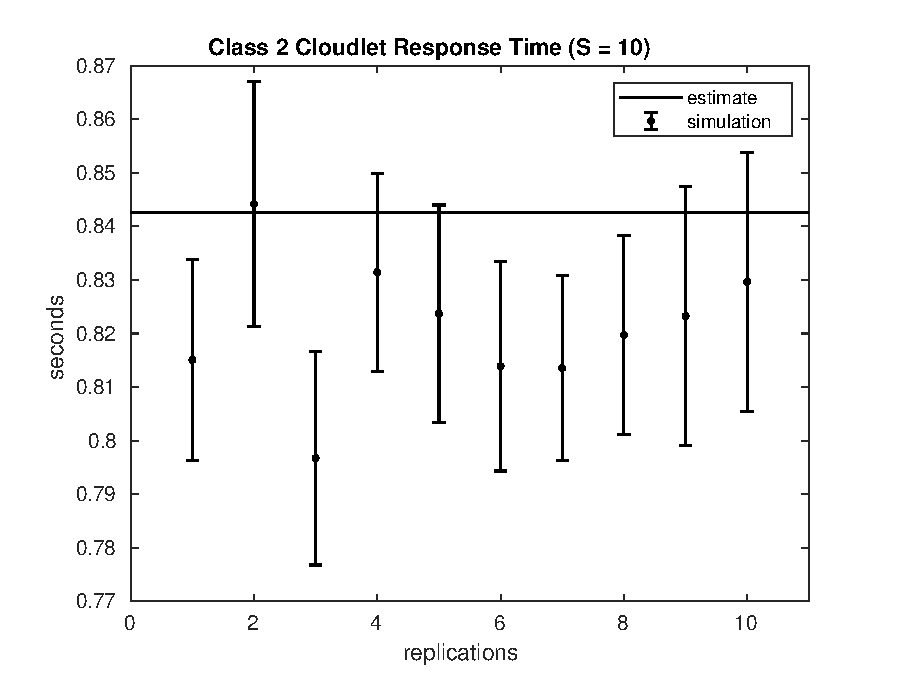
\includegraphics[width=\textwidth]{figures/simul/10_500K_s2clet}
\caption{$S = 10$}
\label{10_s2clet}
\end{subfigure}
%
\begin{subfigure}[t]{0.49\textwidth}
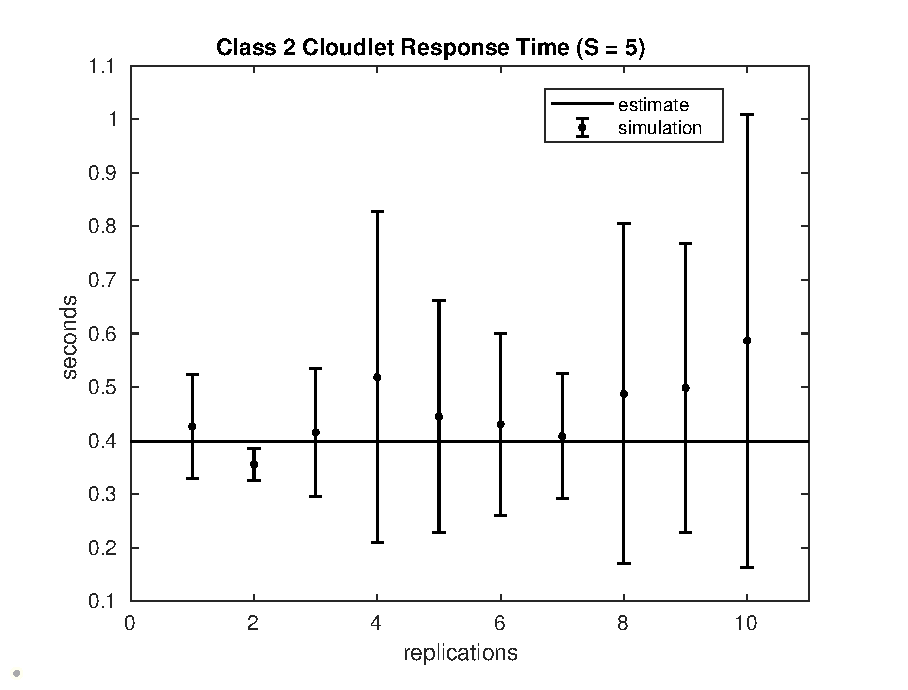
\includegraphics[width=\textwidth]{figures/simul/5_500K_s2clet}
\caption{$S = 5$}
\label{5_s2clet}
\end{subfigure}
%
\caption{tempo di risposta cloudlet classe 2}
\label{plot:s2clet}
\end{figure}
%
%
\begin{table}[!h]
\begin{adjustbox}{width=\textwidth}
\begin{tabular}{c|r@{.}l|r@{.}l|r@{.}l|r@{.}l}
& \multicolumn{2}{|c|}{$S=20$}
& \multicolumn{2}{|c|}{$S=15$}
& \multicolumn{2}{|c|}{$S=10$}
& \multicolumn{2}{|c}{$S=5$}
\\          
\hline
R1      & $2$&$4074 \pm 0.0153$ & $1$&$5819 \pm 0.0184$ & $0$&$8151 \pm 0.0187$ & $0$&$4265 \pm 0.0976$  \\
R2      & $2$&$4115 \pm 0.0172$ & $1$&$6057 \pm 0.0200$ & $0$&$8441 \pm 0.0228$ & $0$&$3558 \pm 0.0302$  \\
R3      & $2$&$3949 \pm 0.0164$ & $1$&$5730 \pm 0.0195$ & $0$&$7968 \pm 0.0199$ & $0$&$4156 \pm 0.1189$  \\
R4      & $2$&$4221 \pm 0.0175$ & $1$&$6014 \pm 0.0173$ & $0$&$8314 \pm 0.0185$ & $0$&$5185 \pm 0.3093$  \\
R5      & $2$&$4125 \pm 0.0172$ & $1$&$5697 \pm 0.0206$ & $0$&$8237 \pm 0.0203$ & $0$&$4449 \pm 0.2161$  \\
R6      & $2$&$3891 \pm 0.0148$ & $1$&$6024 \pm 0.0186$ & $0$&$8139 \pm 0.0196$ & $0$&$4307 \pm 0.1697$  \\
R7      & $2$&$3929 \pm 0.0173$ & $1$&$6096 \pm 0.0178$ & $0$&$8136 \pm 0.0173$ & $0$&$4085 \pm 0.1162$  \\
R8      & $2$&$3962 \pm 0.0168$ & $1$&$6057 \pm 0.0194$ & $0$&$8197 \pm 0.0186$ & $0$&$4874 \pm 0.3175$  \\
R9      & $2$&$4046 \pm 0.0167$ & $1$&$6024 \pm 0.0165$ & $0$&$8232 \pm 0.0241$ & $0$&$4984 \pm 0.2696$  \\
R10     & $2$&$4107 \pm 0.0168$ & $1$&$6139 \pm 0.0155$ & $0$&$8296 \pm 0.0242$ & $0$&$5865 \pm 0.4225$  \\
EST     & $2$&$3904$            & $1$&$6238$            & $0$&$8425$            & $0$&$3980$             \\
\epsmx  & $0$&$0492 \ (2.0\%)$  & $0$&$0336 \ (2.1\%)$  & $0$&$0258 \ (3.2\%)$  & $0$&$6110 \ (104.2\%)$   
\end{tabular}
\end{adjustbox}
\caption{tempo di risposta cloudlet classe 2}
\label{tab:s2clet}
\end{table}

%%%%%%%%%%%%%%%%%%%%%%%%%%%%%%%%%%%%%%%%%%%%%%%%%%%%%%%%%%%%%%%%%%%%%%%%%%%%%%%%%
\subsection{Tempo di Risposta Cloudlet}
I risultati della simulazione (figura~\ref{plot:sclet} e
tabella~\ref{tab:sclet}) mostrano come il clodlet reagisce in base ai diversi
scenari:
\begin{itemize}
\item[$S=5$ :] l'esiguo numero di job di classe 2 processati nel cloudlet
discusso in precedenza, fa sì che nel cloudlet è come se fossero eseguiti
soltanto job di classe 1, infatti il tempo di risposta medio globale del nodo è
molto vicino al tempo di risposta medio di quest'ultimi;
\item[$S=20$ :] in questo caso le interruzioni comportano una riduzione
significativa del tempo di servizio medio dei job di classe 2, pertanto il tempo
di risposta medio globale del cloudlet ne risulta attenuato;
\item[$S=10,15$ :] il maggior numero di interruzioni riduce di molto il tempo di
servizio medio dei job di classe 2, in maniera tale da portare il tempo di
risposta medio globale del cloudlet al di sotto del tempo che si avrebbe nel
caso in cui fossero eseguiti soltanto job di classe 1.
\end{itemize}

Le stime effettuate si avvicinano ai valori delle simulazioni con un errore che
va dallo $0.7\%$ del caso in cui $S=10$ all' $1.7\%$ del caso in cui $S=5$.
Degno di nota è il fatto che, in quest'ultimo caso, l'errore sulla stima della
statistica di classe 2 precedente, non abbia inciso particolarmente, sempre
per via dell'esiguo numero di job processati della suddetta classe.
\begin{figure}[!h]
\centering
%
\begin{subfigure}[t]{0.49\textwidth}
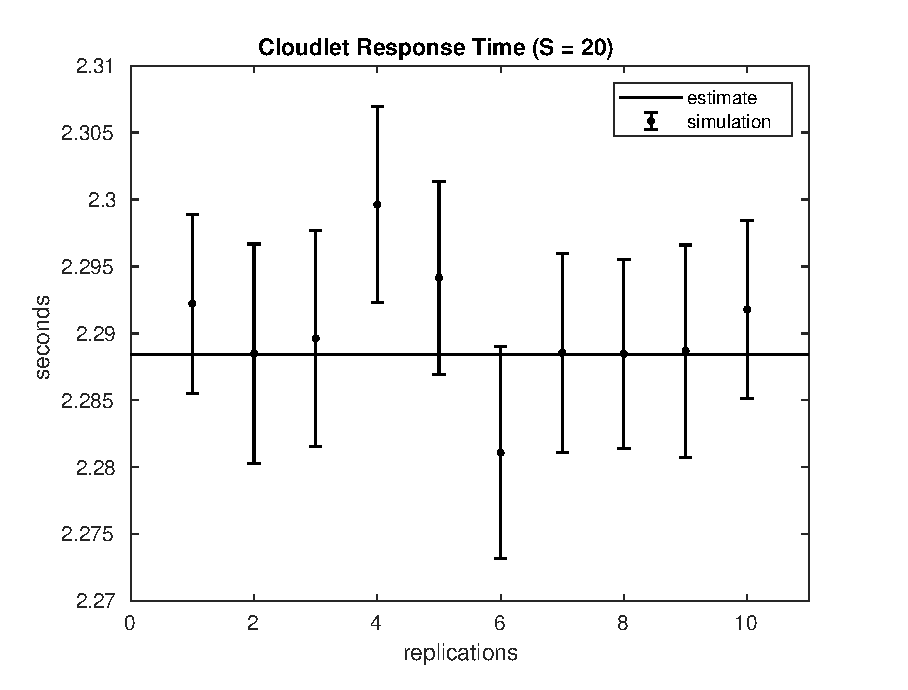
\includegraphics[width=\textwidth]{figures/simul/20_500K_sclet}
\caption{$S = 20$}
\label{20_sclet}
\end{subfigure}
%
\begin{subfigure}[t]{0.49\textwidth}
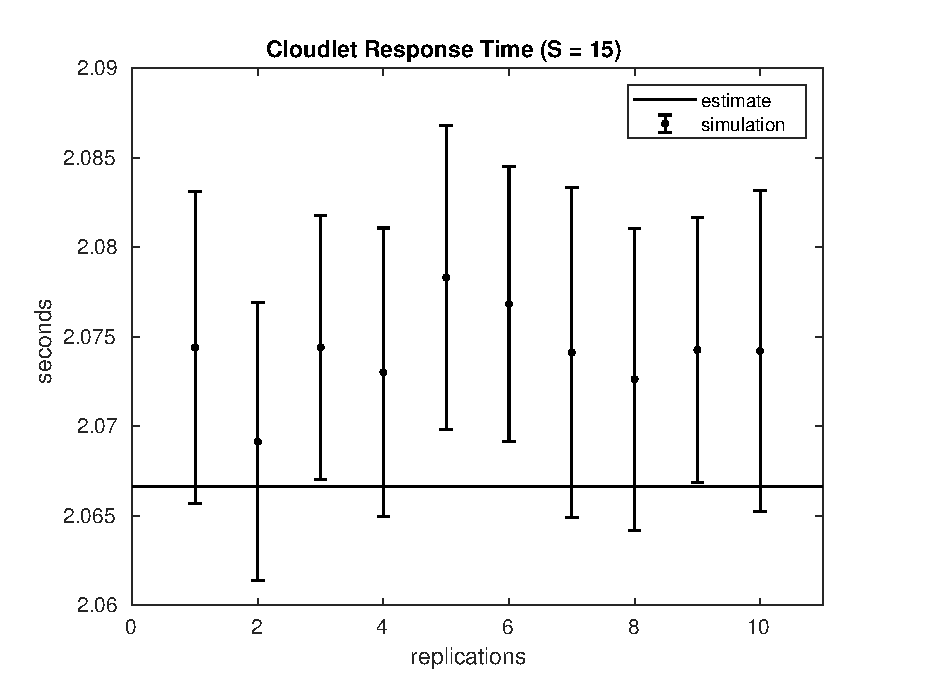
\includegraphics[width=\textwidth]{figures/simul/15_500K_sclet}
\caption{$S = 15$}
\label{15_sclet}
\end{subfigure}
%
\begin{subfigure}[t]{0.49\textwidth}
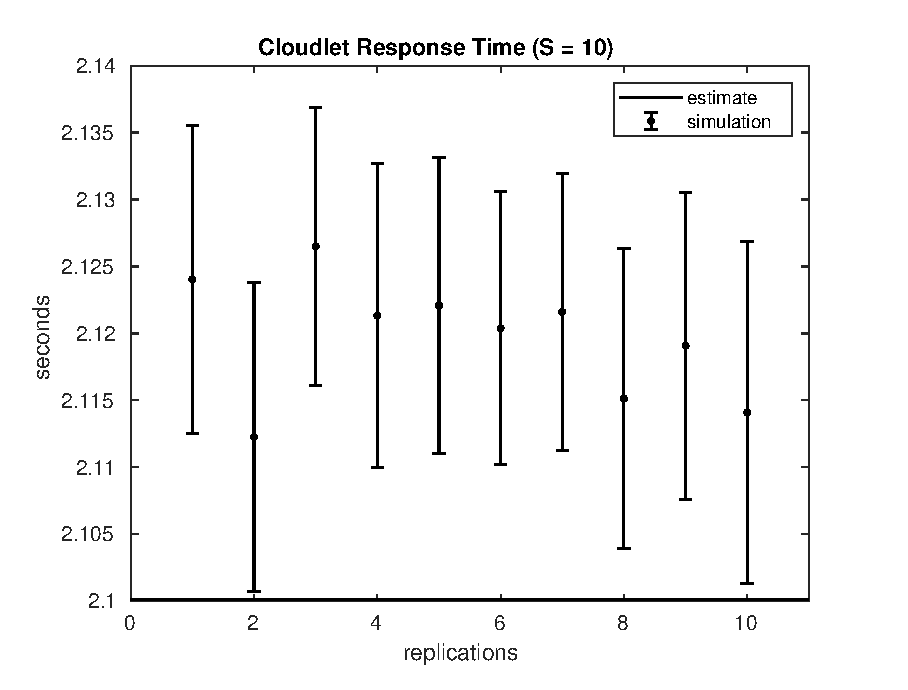
\includegraphics[width=\textwidth]{figures/simul/10_500K_sclet}
\caption{$S = 10$}
\label{10_sclet}
\end{subfigure}
%
\begin{subfigure}[t]{0.49\textwidth}
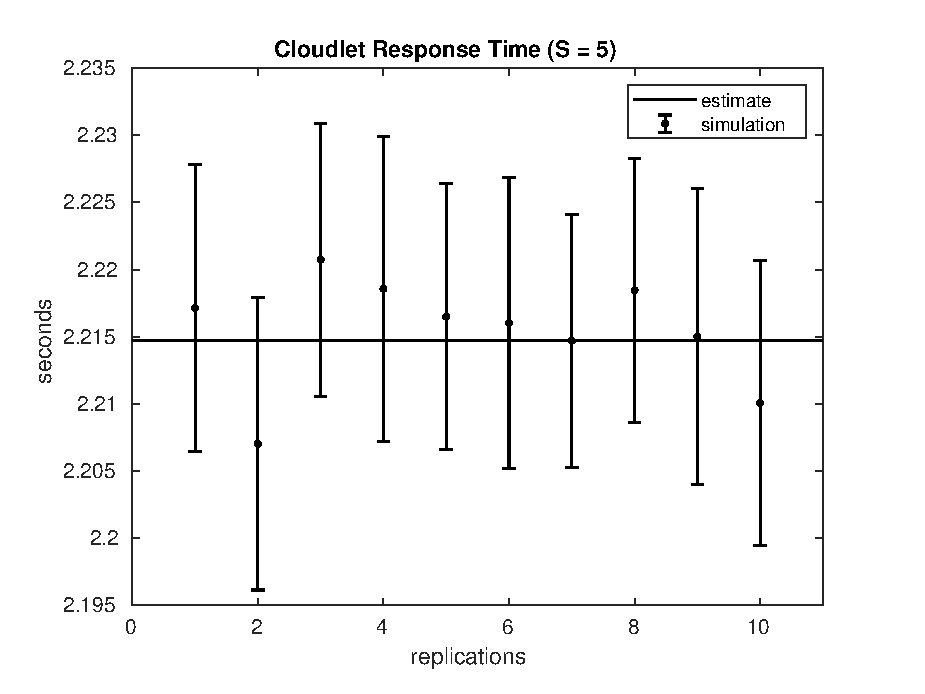
\includegraphics[width=\textwidth]{figures/simul/5_500K_sclet}
\caption{$S = 5$}
\label{5_sclet}
\end{subfigure}
%
\caption{tempo di risposta cloudlet}
\label{plot:sclet}
\end{figure}
%
%
\begin{table}[!h]
\begin{adjustbox}{width=\textwidth}
\begin{tabular}{c|r@{.}l|r@{.}l|r@{.}l|r@{.}l}
& \multicolumn{2}{|c|}{$S=20$}
& \multicolumn{2}{|c|}{$S=15$}
& \multicolumn{2}{|c|}{$S=10$}
& \multicolumn{2}{|c}{$S=5$}
\\          
\hline
R1      & $2$&$2922 \pm 0.0067$ & $2$&$0744 \pm 0.0087$ & $2$&$1240 \pm 0.0115$ & $2$&$2171 \pm 0.0107$ \\
R2      & $2$&$2885 \pm 0.0082$ & $2$&$0691 \pm 0.0078$ & $2$&$1123 \pm 0.0115$ & $2$&$2070 \pm 0.0109$ \\
R3      & $2$&$2896 \pm 0.0081$ & $2$&$0744 \pm 0.0074$ & $2$&$1265 \pm 0.0104$ & $2$&$2207 \pm 0.0102$ \\
R4      & $2$&$2996 \pm 0.0073$ & $2$&$0730 \pm 0.0081$ & $2$&$1213 \pm 0.0114$ & $2$&$2186 \pm 0.0113$ \\
R5      & $2$&$2942 \pm 0.0072$ & $2$&$0783 \pm 0.0085$ & $2$&$1221 \pm 0.0110$ & $2$&$2165 \pm 0.0099$ \\
R6      & $2$&$2811 \pm 0.0079$ & $2$&$0768 \pm 0.0077$ & $2$&$1204 \pm 0.0102$ & $2$&$2160 \pm 0.0108$ \\
R7      & $2$&$2885 \pm 0.0074$ & $2$&$0741 \pm 0.0092$ & $2$&$1216 \pm 0.0103$ & $2$&$2147 \pm 0.0094$ \\
R8      & $2$&$2885 \pm 0.0071$ & $2$&$0726 \pm 0.0084$ & $2$&$1151 \pm 0.0112$ & $2$&$2185 \pm 0.0098$ \\
R9      & $2$&$2887 \pm 0.0079$ & $2$&$0743 \pm 0.0074$ & $2$&$1191 \pm 0.0115$ & $2$&$2150 \pm 0.0110$ \\
R10     & $2$&$2918 \pm 0.0066$ & $2$&$0742 \pm 0.0090$ & $2$&$1141 \pm 0.0127$ & $2$&$2101 \pm 0.0106$ \\
EST     & $2$&$2884$            & $2$&$0666$            & $2$&$1002$            & $2$&$2147$            \\
\epsmx  & $0$&$0185 \ (0.8\%)$  & $0$&$0201 \ (1.0\%)$  & $0$&$0367 \ (1.7\%)$  & $0$&$0162 \ (0.7\%)$    
\end{tabular}
\end{adjustbox}
\caption{tempo di risposta cloudlet}
\label{tab:sclet}
\end{table}

%%%%%%%%%%%%%%%%%%%%%%%%%%%%%%%%%%%%%%%%%%%%%%%%%%%%%%%%%%%%%%%%%%%%%%%%%%%%%%%%
\subsection{Tempo di Risposta Cloud Classe 2}
Il tempo di risposta per un job di classe 2 che viene eseguito nel cloud è
indipendente dal parametro S ed i risultati presentati in
figura~\ref{plot:s2cloud} e nella tabella~\ref{tab:s2cloud} mostrano che tutti
gli intervalli di confidenza calcolati comprendono il valore stimato ed il
valore dell'errore massimo è sotto la soglia dell'$1\%$ in ogni caso.
\begin{figure}[!h]
\centering
%
\begin{subfigure}[t]{0.49\textwidth}
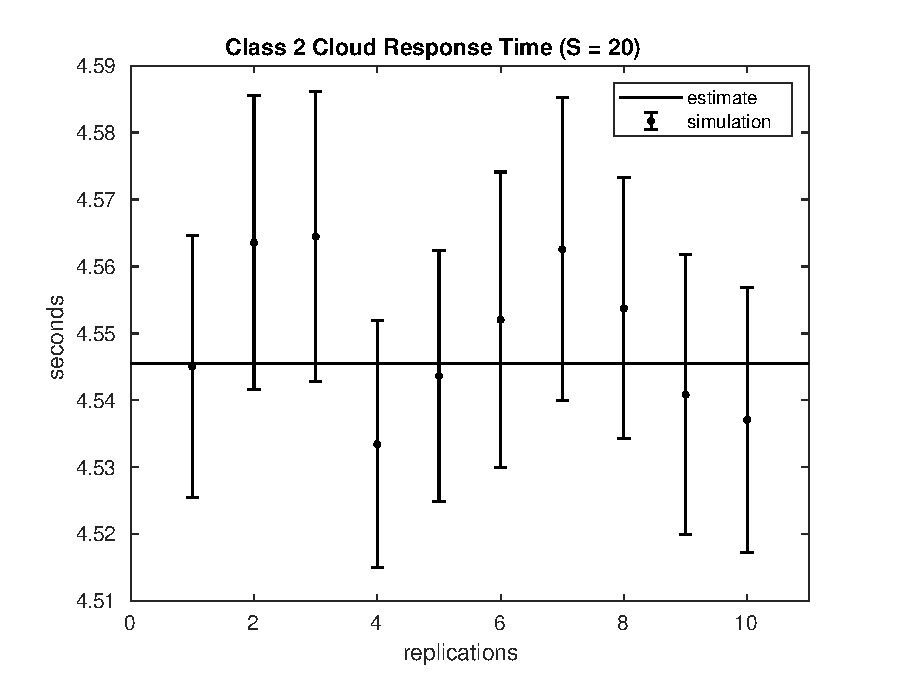
\includegraphics[width=\textwidth]{figures/simul/20_500K_s2cloud}
\caption{$S = 20$}
\label{20_s2cloud}
\end{subfigure}
%
\begin{subfigure}[t]{0.49\textwidth}
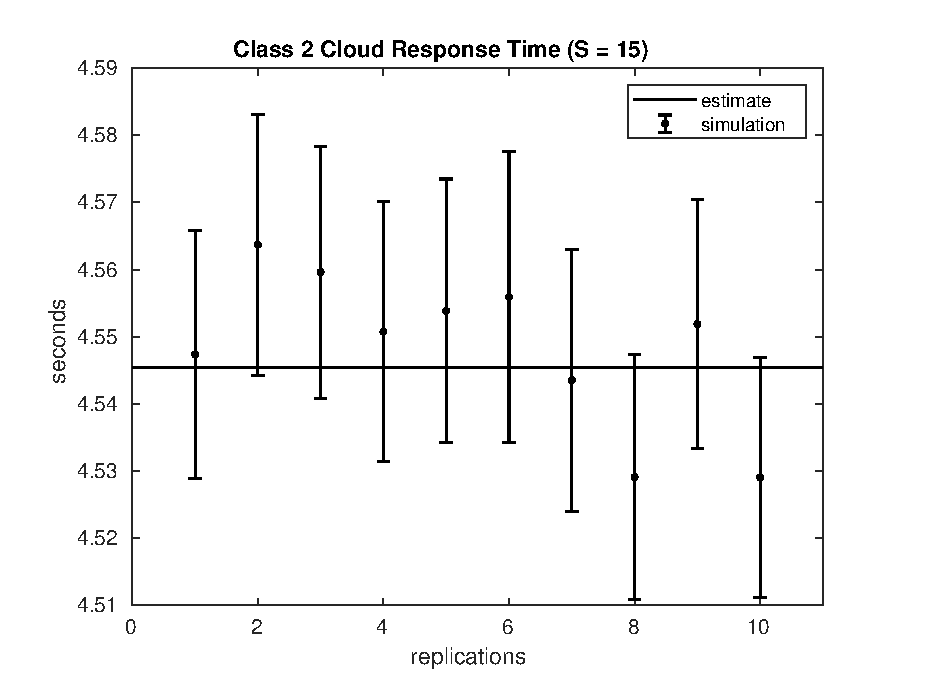
\includegraphics[width=\textwidth]{figures/simul/15_500K_s2cloud}
\caption{$S = 15$}
\label{15_s2cloud}
\end{subfigure}
%
\begin{subfigure}[t]{0.49\textwidth}
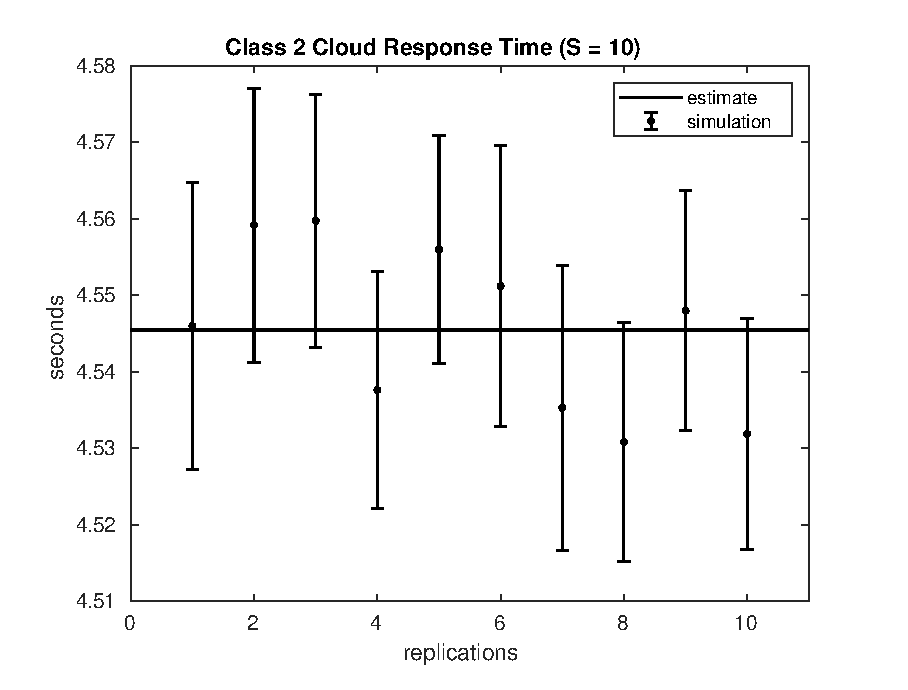
\includegraphics[width=\textwidth]{figures/simul/10_500K_s2cloud}
\caption{$S = 10$}
\label{10_s2cloud}
\end{subfigure}
%
\begin{subfigure}[t]{0.49\textwidth}
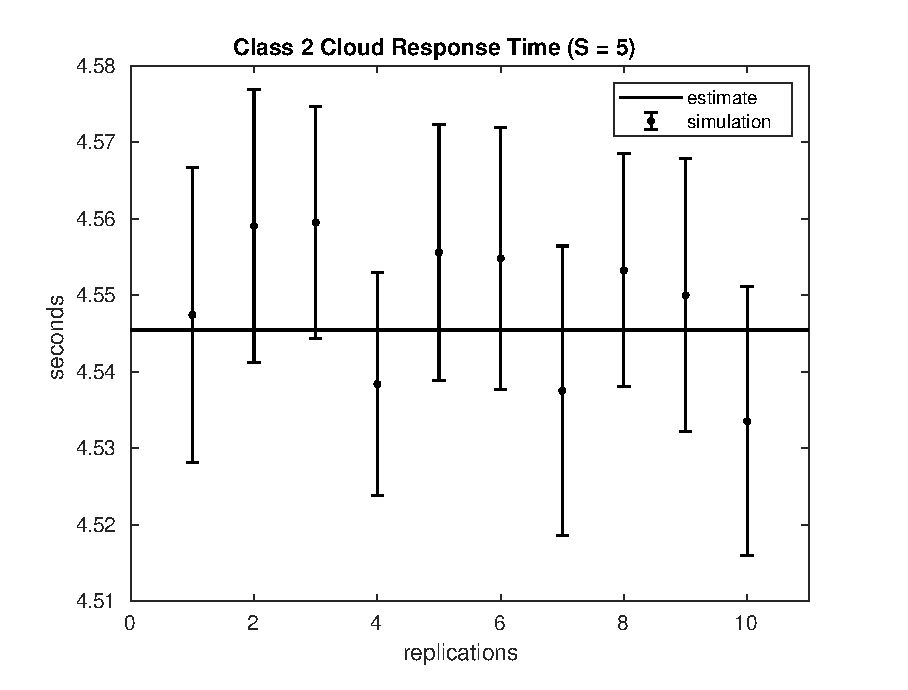
\includegraphics[width=\textwidth]{figures/simul/5_500K_s2cloud}
\caption{$S = 5$}
\label{5_s2cloud}
\end{subfigure}
%
\caption{tempo di risposta cloud classe 2}
\label{plot:s2cloud}
\end{figure}
%
%
\begin{table}[!h]
\begin{adjustbox}{width=\textwidth}
\begin{tabular}{c|r@{.}l|r@{.}l|r@{.}l|r@{.}l}
& \multicolumn{2}{|c|}{$S=20$}
& \multicolumn{2}{|c|}{$S=15$} 
& \multicolumn{2}{|c|}{$S=10$} 
& \multicolumn{2}{|c}{$S=5$} 
\\          
\hline
R1      & $4$&$5450 \pm 0.0196$  & $4$&$5474 \pm 0.0184$ & $4$&$5460 \pm 0.0188$ & $4$&$5474 \pm 0.0192$ \\
R2      & $4$&$5636 \pm 0.0219$  & $4$&$5637 \pm 0.0194$ & $4$&$5591 \pm 0.0179$ & $4$&$5590 \pm 0.0179$ \\
R3      & $4$&$5644 \pm 0.0216$  & $4$&$5596 \pm 0.0188$ & $4$&$5597 \pm 0.0165$ & $4$&$5595 \pm 0.0152$ \\
R4      & $4$&$5335 \pm 0.0185$  & $4$&$5507 \pm 0.0193$ & $4$&$5376 \pm 0.0154$ & $4$&$5384 \pm 0.0146$ \\
R5      & $4$&$5436 \pm 0.0187$  & $4$&$5538 \pm 0.0196$ & $4$&$5560 \pm 0.0148$ & $4$&$5556 \pm 0.0168$ \\
R6      & $4$&$5520 \pm 0.0221$  & $4$&$5559 \pm 0.0216$ & $4$&$5512 \pm 0.0183$ & $4$&$5548 \pm 0.0171$ \\
R7      & $4$&$5626 \pm 0.0226$  & $4$&$5435 \pm 0.0195$ & $4$&$5353 \pm 0.0186$ & $4$&$5375 \pm 0.0189$ \\
R8      & $4$&$5537 \pm 0.0195$  & $4$&$5291 \pm 0.0182$ & $4$&$5308 \pm 0.0156$ & $4$&$5533 \pm 0.0152$ \\
R9      & $4$&$5409 \pm 0.0209$  & $4$&$5519 \pm 0.0185$ & $4$&$5480 \pm 0.0157$ & $4$&$5500 \pm 0.0178$ \\
R10     & $4$&$5371 \pm 0.0197$  & $4$&$5291 \pm 0.0179$ & $4$&$5319 \pm 0.0151$ & $4$&$5335 \pm 0.0176$ \\
EST     & $4$&$5455$             & $4$&$5455$            & $4$&$5455$            & $4$&$5455$            \\
\epsmx  & $0$&$0406 \ (0.9\%)$   & $0$&$0376 \ (0.8\%)$  & $0$&$0316 \ (0.7\%)$  & $0$&$0314 \ (0.7\%)$    
\end{tabular}
\end{adjustbox}
\caption{tempo di risposta cloud classe 2}
\label{tab:s2cloud}
\end{table}

%%%%%%%%%%%%%%%%%%%%%%%%%%%%%%%%%%%%%%%%%%%%%%%%%%%%%%%%%%%%%%%%%%%%%%%%%%%%%%%%%
\subsection{Tempo di Risposta Cloud}
Il tempo di risposta del cloud è completamente dominato dai job di classe 2,
infatti, come mostrano la figura~\ref{plot:scloud} e la
tabella~\ref{tab:scloud}, i risultati sono pressoché identici alla precedente
metrica.
\begin{figure}[!h]
\centering
%
\begin{subfigure}[t]{0.49\textwidth}
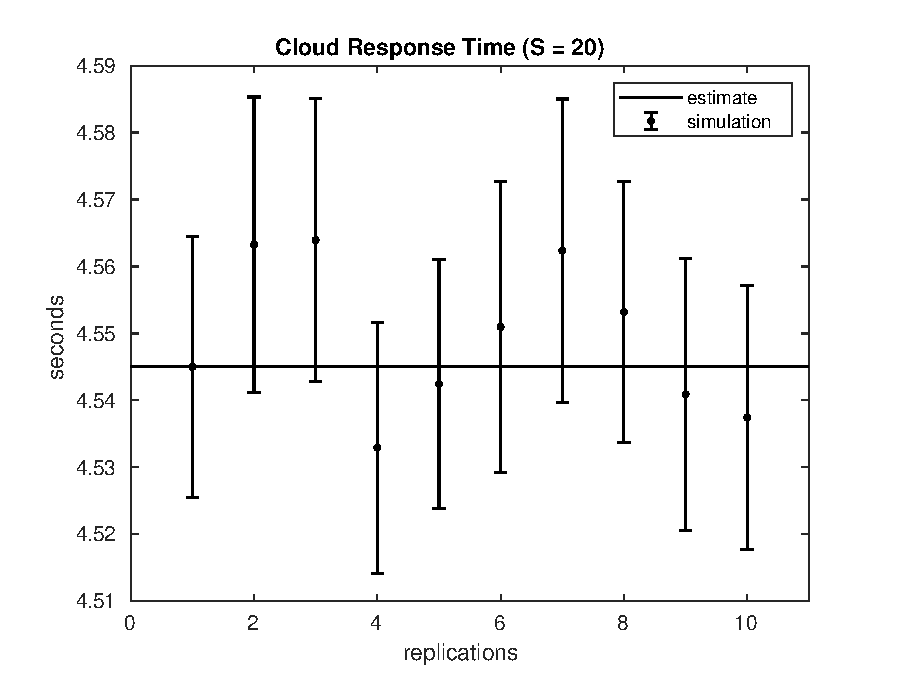
\includegraphics[width=\textwidth]{figures/simul/20_500K_scloud}
\caption{$S = 20$}
\label{20_scloud}
\end{subfigure}
%
\begin{subfigure}[t]{0.49\textwidth}
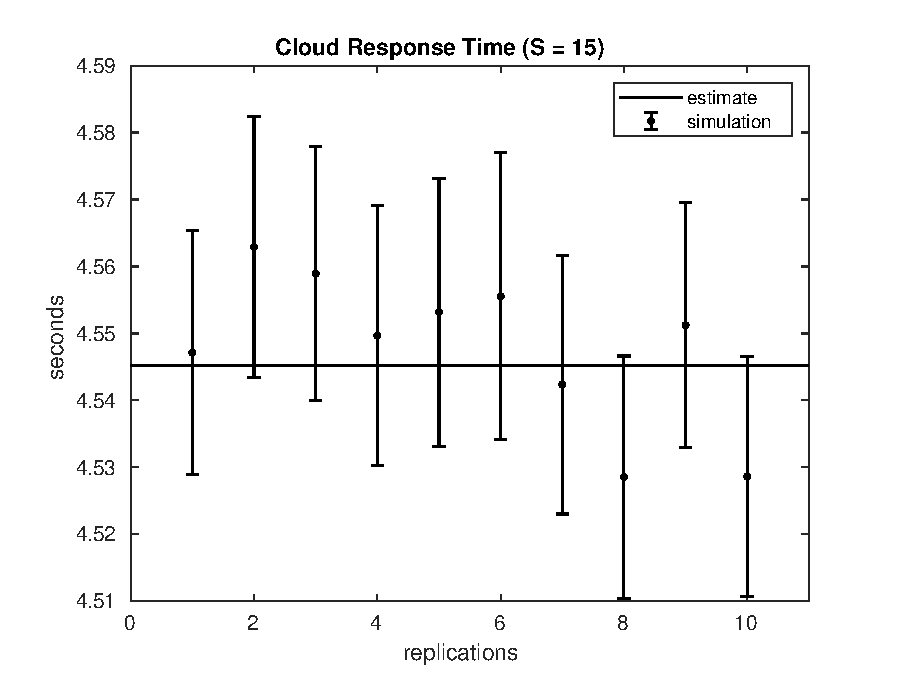
\includegraphics[width=\textwidth]{figures/simul/15_500K_scloud}
\caption{$S = 15$}
\label{15_scloud}
\end{subfigure}
%
\begin{subfigure}[t]{0.49\textwidth}
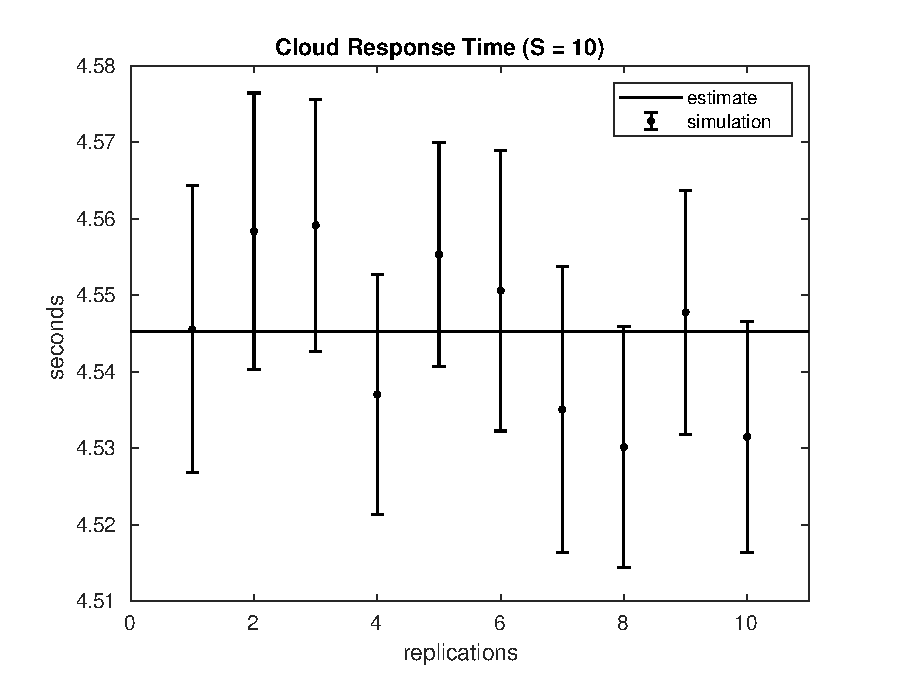
\includegraphics[width=\textwidth]{figures/simul/10_500K_scloud}
\caption{$S = 10$}
\label{10_scloud}
\end{subfigure}
%
\begin{subfigure}[t]{0.49\textwidth}
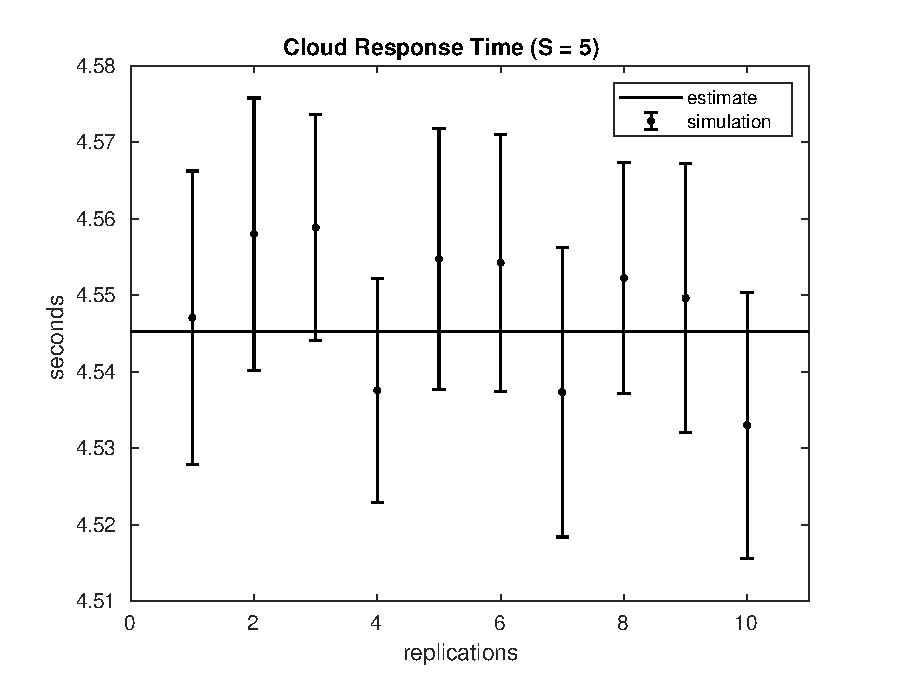
\includegraphics[width=\textwidth]{figures/simul/5_500K_scloud}
\caption{$S = 5$}
\label{5_scloud}
\end{subfigure}
%
\caption{tempo di risposta cloud}
\label{plot:scloud}
\end{figure}
%
%
\begin{table}[!h]
\begin{adjustbox}{width=\textwidth}
\begin{tabular}{c|r@{.}l|r@{.}l|r@{.}l|r@{.}l}
& \multicolumn{2}{|c|}{$S=20$}
& \multicolumn{2}{|c|}{$S=15$} 
& \multicolumn{2}{|c|}{$S=10$} 
& \multicolumn{2}{|c}{$S=5$} 
\\          
\hline
R1      & $4$&$5450 \pm 0.0195$ & $4$&$5471 \pm 0.0182$ & $4$&$5455 \pm 0.0187$ & $4$&$5471 \pm 0.0192$ \\
R2      & $4$&$5633 \pm 0.0220$ & $4$&$5629 \pm 0.0195$ & $4$&$5583 \pm 0.0181$ & $4$&$5580 \pm 0.0178$ \\
R3      & $4$&$5639 \pm 0.0211$ & $4$&$5589 \pm 0.0189$ & $4$&$5591 \pm 0.0164$ & $4$&$5588 \pm 0.0147$ \\
R4      & $4$&$5329 \pm 0.0188$ & $4$&$5497 \pm 0.0194$ & $4$&$5370 \pm 0.0157$ & $4$&$5376 \pm 0.0146$ \\
R5      & $4$&$5424 \pm 0.0185$ & $4$&$5532 \pm 0.0200$ & $4$&$5553 \pm 0.0146$ & $4$&$5548 \pm 0.0170$ \\
R6      & $4$&$5510 \pm 0.0217$ & $4$&$5555 \pm 0.0214$ & $4$&$5506 \pm 0.0183$ & $4$&$5542 \pm 0.0168$ \\
R7      & $4$&$5624 \pm 0.0226$ & $4$&$5424 \pm 0.0193$ & $4$&$5351 \pm 0.0186$ & $4$&$5373 \pm 0.0189$ \\
R8      & $4$&$5532 \pm 0.0195$ & $4$&$5286 \pm 0.0181$ & $4$&$5301 \pm 0.0158$ & $4$&$5523 \pm 0.0151$ \\
R9      & $4$&$5409 \pm 0.0204$ & $4$&$5512 \pm 0.0183$ & $4$&$5478 \pm 0.0159$ & $4$&$5496 \pm 0.0175$ \\
R10     & $4$&$5374 \pm 0.0197$ & $4$&$5287 \pm 0.0179$ & $4$&$5315 \pm 0.0151$ & $4$&$5330 \pm 0.0174$ \\
EST     & $4$&$5451$            & $4$&$5452$            & $4$&$5453$            & $4$&$5453$            \\
\epsmx  & $0$&$0402 \ (0.9\%)$  & $0$&$0372 \ (0.8\%)$  & $0$&$0312 \ (0.7\%)$  & $0$&$0305 \ (0.7\%)$    
\end{tabular}
\end{adjustbox}
\caption{tempo di risposta cloud}
\label{tab:scloud}
\end{table}

%%%%%%%%%%%%%%%%%%%%%%%%%%%%%%%%%%%%%%%%%%%%%%%%%%%%%%%%%%%%%%%%%%%%%%%%%%%%%%%%
\subsection{Tempo di Risposta Job Interrotti}
La figura~\ref{plot:sintr} e la tabella~\ref{tab:sintr}, confermano che il tempo
di risposta dei job interrotti ha un andamento analogo al tempo di risposta
medio dei job di classe 2 processati con successo nel cloudlet, infatti si nota
che tale tempo è direttamente proporzionale al parametro di soglia, quindi
inversamente proporzionale alla probabilità di interruzione.

Effettuando un confronto con i tempi di risposta del cloudlet, ci si rende conto
di quanto costi l'interruzione di un job ed è quindi lecito aspettarsi che
queste interruzioni incidano in maniera significativa sul tempo di risposta dei
job di classe 2 del sistema.

Anche l'errore massimo che si è commesso con la stima della statistiche, sembra
crescere con $S$, infatti per $S=5$ si ha un errore massimo dell'$1.1\%$ che
cresce fino ad arrivare al $2.5\%$ nel caso in cui $S=20$. 
\begin{figure}[!h]
\centering
%
\begin{subfigure}[t]{0.49\textwidth}
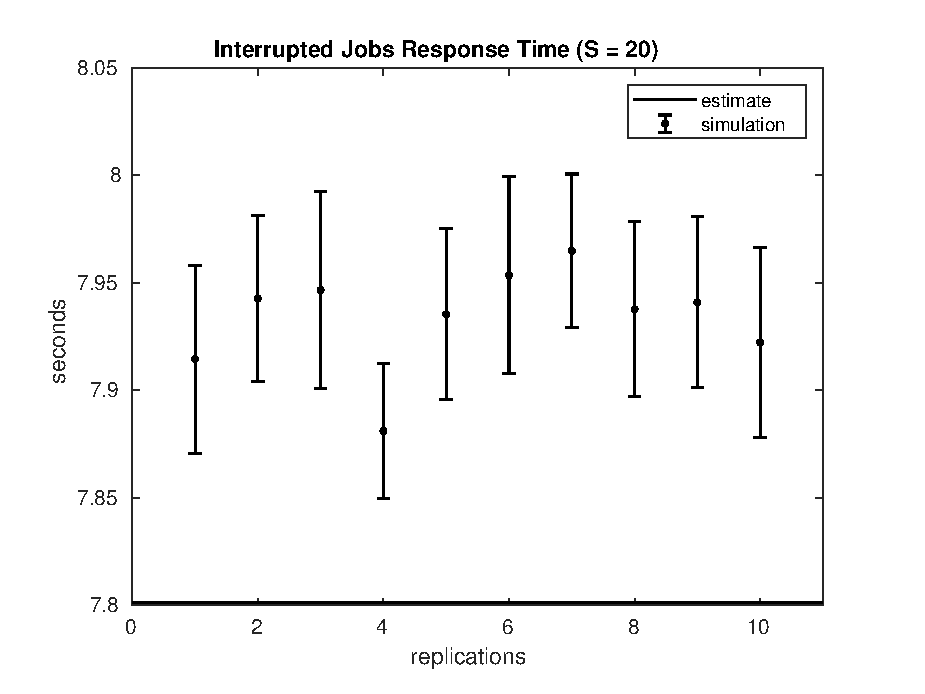
\includegraphics[width=\textwidth]{figures/simul/20_500K_sintr}
\caption{$S = 20$}
\label{20_sintr}
\end{subfigure}
%
\begin{subfigure}[t]{0.49\textwidth}
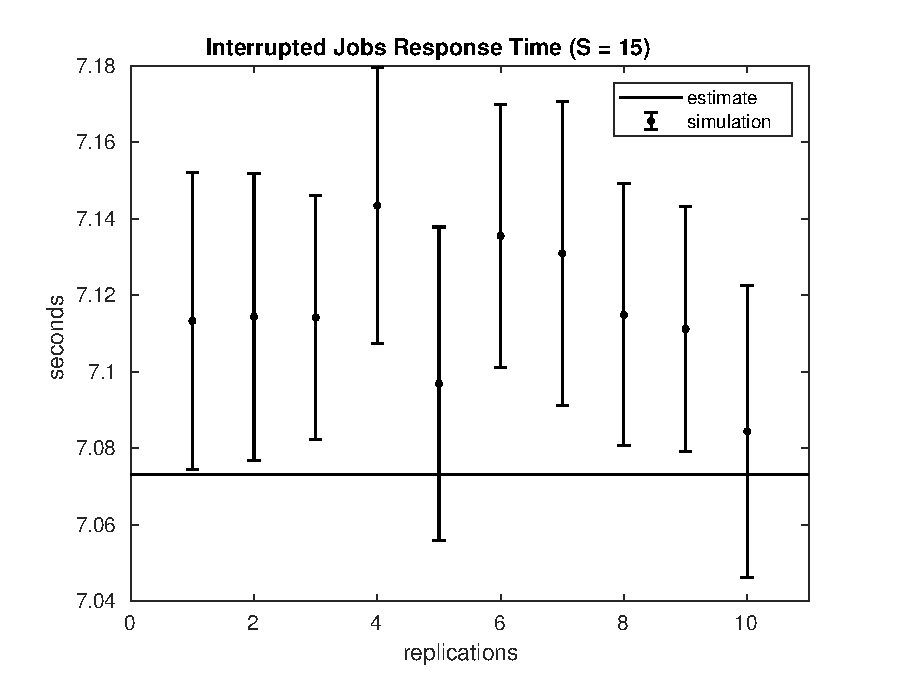
\includegraphics[width=\textwidth]{figures/simul/15_500K_sintr}
\caption{$S = 15$}
\label{15_sintr}
\end{subfigure}
%
\begin{subfigure}[t]{0.49\textwidth}
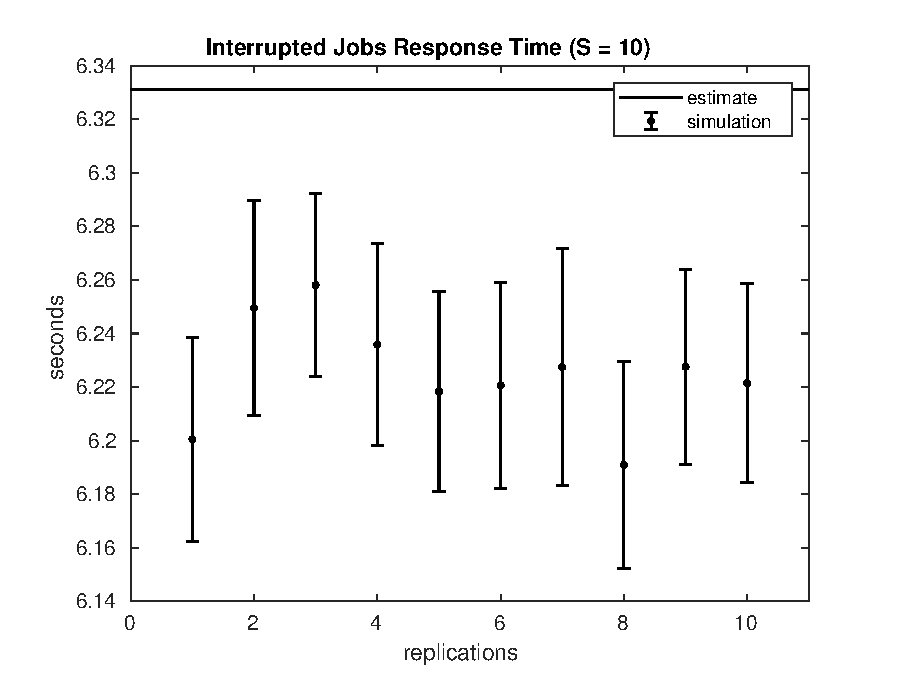
\includegraphics[width=\textwidth]{figures/simul/10_500K_sintr}
\caption{$S = 10$}
\label{10_sintr}
\end{subfigure}
%
\begin{subfigure}[t]{0.49\textwidth}
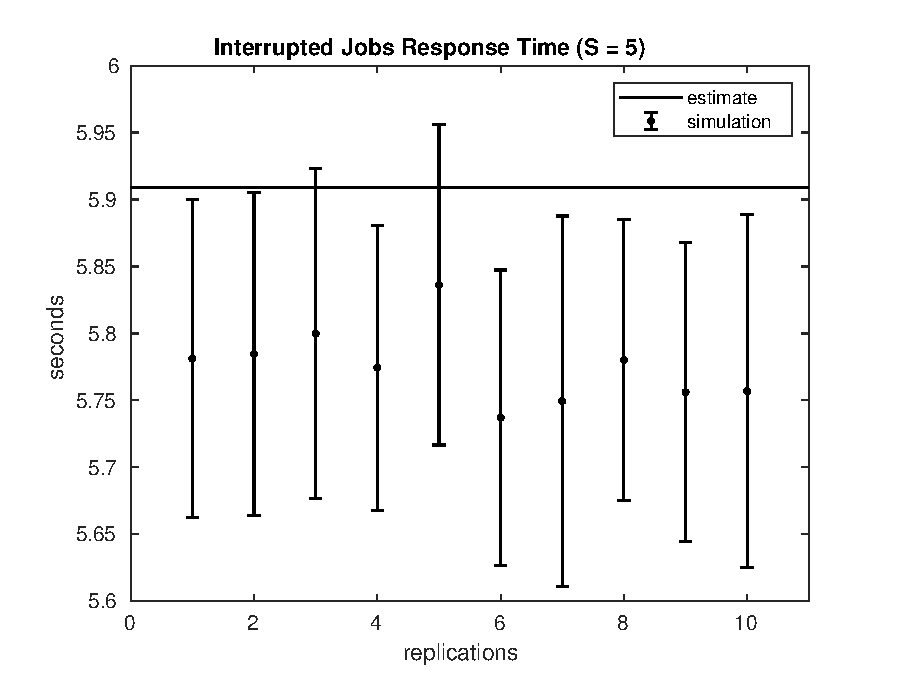
\includegraphics[width=\textwidth]{figures/simul/5_500K_sintr}
\caption{$S = 5$}
\label{5_sintr}
\end{subfigure}
%
\caption{tempo di risposta job interrotti}
\label{plot:sintr}
\end{figure}
%
%
\begin{table}[!h]
\begin{adjustbox}{width=\textwidth}
\begin{tabular}{c|r@{.}l|r@{.}l|r@{.}l|r@{.}l}
& \multicolumn{2}{|c|}{$S=20$}
& \multicolumn{2}{|c|}{$S=15$} 
& \multicolumn{2}{|c|}{$S=10$} 
& \multicolumn{2}{|c}{$S=5$} 
\\          
\hline
R1      & $7$&$9146 \pm 0.0437$  & $7$&$1133 \pm 0.0388$ & $6$&$2006 \pm 0.0381$ & $5$&$7813 \pm 0.1190$ \\
R2      & $7$&$9427 \pm 0.0387$  & $7$&$1144 \pm 0.0374$ & $6$&$2496 \pm 0.0401$ & $5$&$7846 \pm 0.1207$ \\
R3      & $7$&$9467 \pm 0.0458$  & $7$&$1142 \pm 0.0319$ & $6$&$2580 \pm 0.0342$ & $5$&$7998 \pm 0.1230$ \\
R4      & $7$&$8812 \pm 0.0312$  & $7$&$1434 \pm 0.0361$ & $6$&$2358 \pm 0.0377$ & $5$&$7744 \pm 0.1065$ \\
R5      & $7$&$9354 \pm 0.0398$  & $7$&$0969 \pm 0.0409$ & $6$&$2184 \pm 0.0373$ & $5$&$8362 \pm 0.1194$ \\
R6      & $7$&$9536 \pm 0.0457$  & $7$&$1355 \pm 0.0343$ & $6$&$2206 \pm 0.0383$ & $5$&$7372 \pm 0.1102$ \\
R7      & $7$&$9649 \pm 0.0358$  & $7$&$1309 \pm 0.0398$ & $6$&$2275 \pm 0.0441$ & $5$&$7496 \pm 0.1381$ \\
R8      & $7$&$9377 \pm 0.0407$  & $7$&$1149 \pm 0.0343$ & $6$&$1910 \pm 0.0386$ & $5$&$7802 \pm 0.1045$ \\
R9      & $7$&$9410 \pm 0.0397$  & $7$&$1112 \pm 0.0319$ & $6$&$2276 \pm 0.0365$ & $5$&$7562 \pm 0.1116$ \\
R10     & $7$&$9223 \pm 0.0443$  & $7$&$0844 \pm 0.0381$ & $6$&$2215 \pm 0.0372$ & $5$&$7570 \pm 0.1319$ \\
EST     & $7$&$8016$             & $7$&$0733$            & $6$&$3310$            & $5$&$9087$            \\
\epsmx  & $0$&$1991 \ (2.5\%)$   & $0$&$1062 \ (1.5\%)$  & $0$&$1015 \ (1.6\%)$  & $0$&$0614 \ (1.1\%)$    
\end{tabular}
\end{adjustbox}
\caption{tempo di risposta job interrotti}
\label{tab:sintr}
\end{table}

%%%%%%%%%%%%%%%%%%%%%%%%%%%%%%%%%%%%%%%%%%%%%%%%%%%%%%%%%%%%%%%%%%%%%%%%%%%%%%%%
\subsection{Tempo di Risposta Sistema Classe 1}
Il tempo di risposta globale dei job di classe 1 è completamente dominato dal
tempo di risposta dei job processati nel cloudlet, essendo molto minore il
numero di quelli eseguiti nel cloud. Infatti la figura~\ref{plot:s1} e la
tabella~\ref{tab:s1} mostrano delle statistiche pressoché identiche a quelle
relative al tempo di risposta dei job di classe 1 eseguiti nel coudlet, con un
errore massimo inferiore all'$1\%$.
\begin{figure}[!h]
\centering
%
\begin{subfigure}[t]{0.49\textwidth}
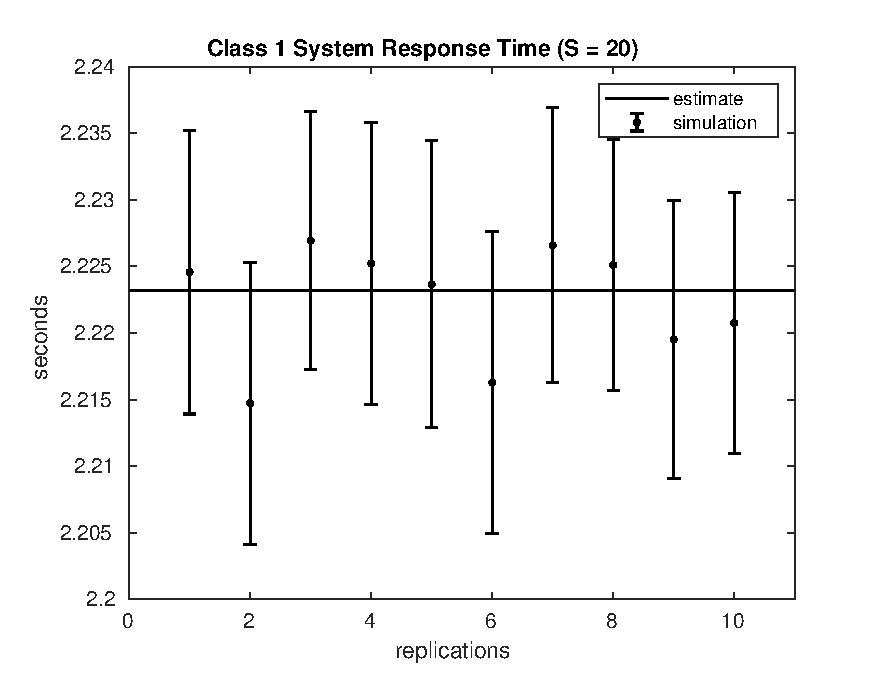
\includegraphics[width=\textwidth]{figures/simul/20_500K_s1}
\caption{$S = 20$}
\label{20_s1}
\end{subfigure}
%
\begin{subfigure}[t]{0.49\textwidth}
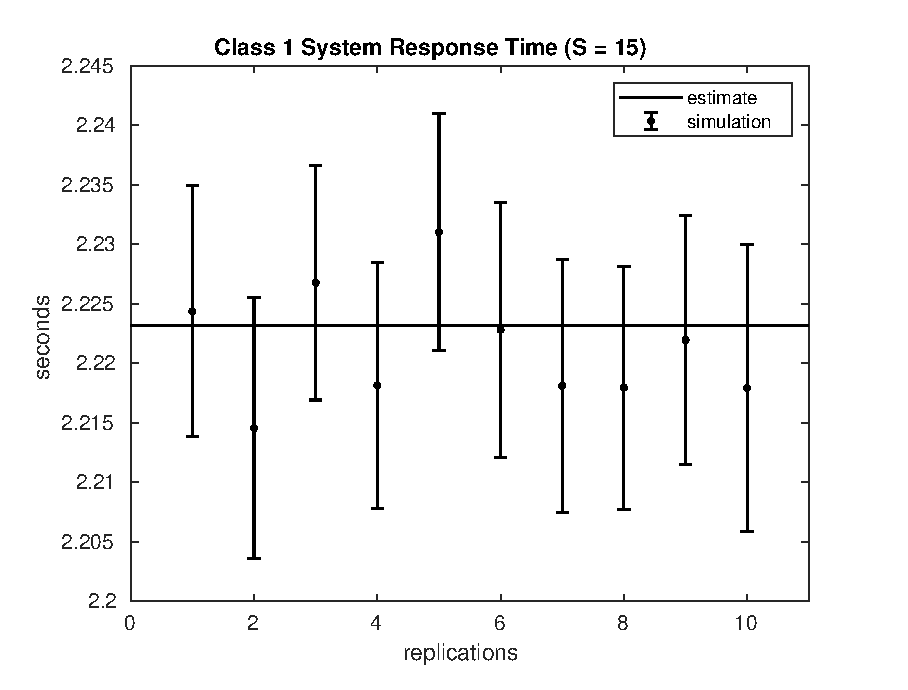
\includegraphics[width=\textwidth]{figures/simul/15_500K_s1}
\caption{$S = 15$}
\label{15_s1}
\end{subfigure}
%
\begin{subfigure}[t]{0.49\textwidth}
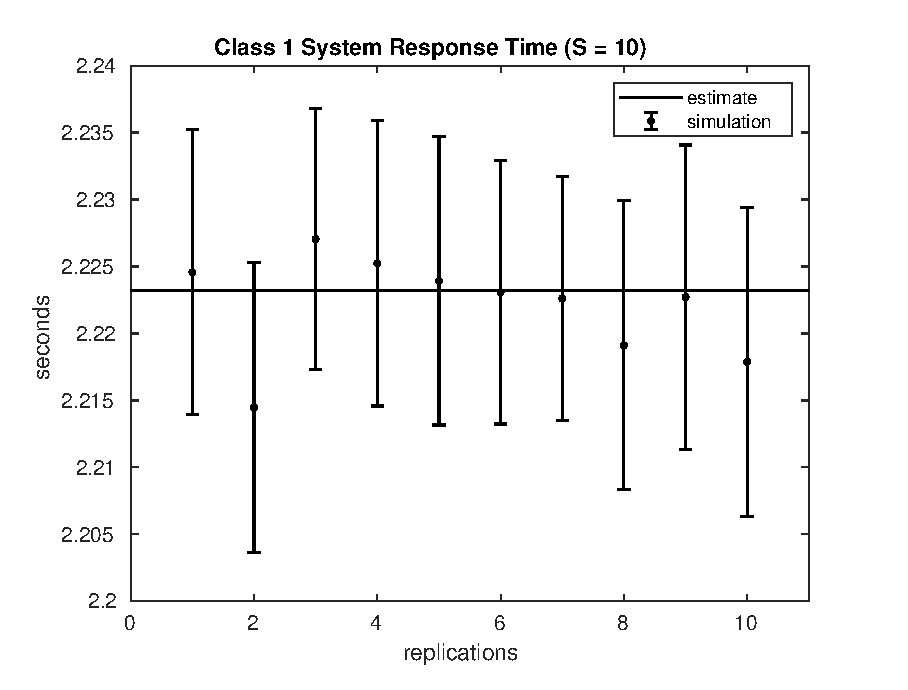
\includegraphics[width=\textwidth]{figures/simul/10_500K_s1}
\caption{$S = 10$}
\label{10_s1}
\end{subfigure}
%
\begin{subfigure}[t]{0.49\textwidth}
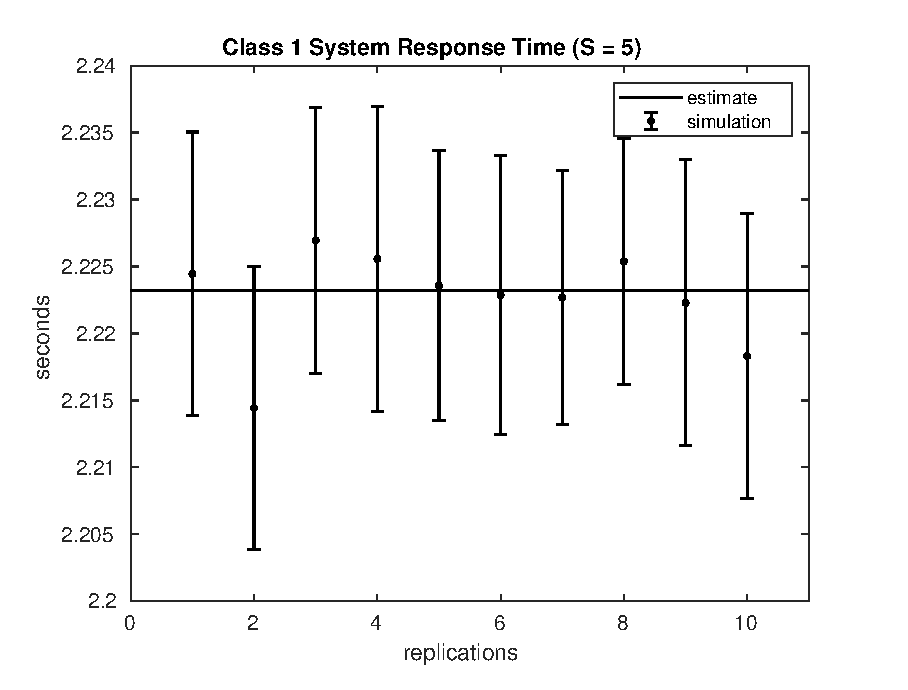
\includegraphics[width=\textwidth]{figures/simul/5_500K_s1}
\caption{$S = 5$}
\label{5_s1}
\end{subfigure}
%
\caption{tempo di risposta sistema classe 1}
\label{plot:s1}
\end{figure}
%
%
\begin{table}[!h]
\begin{adjustbox}{width=\textwidth}
\begin{tabular}{c|r@{.}l|r@{.}l|r@{.}l|r@{.}l}
& \multicolumn{2}{|c|}{$S=20$}
& \multicolumn{2}{|c|}{$S=15$} 
& \multicolumn{2}{|c|}{$S=10$} 
& \multicolumn{2}{|c}{$S=5$} 
\\          
\hline
R1      & $2$&$2246 \pm 0.0107$ & $2$&$2244 \pm 0.0105$ & $2$&$2246 \pm 0.0107$ & $2$&$2245 \pm 0.0106$ \\
R2      & $2$&$2147 \pm 0.0106$ & $2$&$2145 \pm 0.0110$ & $2$&$2145 \pm 0.0108$ & $2$&$2144 \pm 0.0106$ \\
R3      & $2$&$2269 \pm 0.0097$ & $2$&$2268 \pm 0.0098$ & $2$&$2270 \pm 0.0098$ & $2$&$2270 \pm 0.0099$ \\
R4      & $2$&$2252 \pm 0.0106$ & $2$&$2181 \pm 0.0103$ & $2$&$2252 \pm 0.0106$ & $2$&$2256 \pm 0.0114$ \\
R5      & $2$&$2237 \pm 0.0108$ & $2$&$2310 \pm 0.0100$ & $2$&$2239 \pm 0.0108$ & $2$&$2236 \pm 0.0101$ \\
R6      & $2$&$2163 \pm 0.0113$ & $2$&$2228 \pm 0.0107$ & $2$&$2231 \pm 0.0098$ & $2$&$2229 \pm 0.0104$ \\
R7      & $2$&$2266 \pm 0.0103$ & $2$&$2181 \pm 0.0106$ & $2$&$2226 \pm 0.0091$ & $2$&$2227 \pm 0.0095$ \\
R8      & $2$&$2251 \pm 0.0094$ & $2$&$2180 \pm 0.0102$ & $2$&$2191 \pm 0.0108$ & $2$&$2254 \pm 0.0092$ \\
R9      & $2$&$2195 \pm 0.0104$ & $2$&$2220 \pm 0.0104$ & $2$&$2227 \pm 0.0114$ & $2$&$2223 \pm 0.0107$ \\
R10     & $2$&$2208 \pm 0.0098$ & $2$&$2179 \pm 0.0120$ & $2$&$2179 \pm 0.0115$ & $2$&$2183 \pm 0.0107$ \\
EST     & $2$&$2232$            & $2$&$2232$            & $2$&$2232$            & $2$&$2232$            \\
\epsmx  & $0$&$0137 \ (0.6\%)$  & $0$&$0178 \ (0.8\%)$  & $0$&$0136 \ (0.6\%)$  & $0$&$0138 \ (0.6\%)$    
\end{tabular}
\end{adjustbox}
\caption{tempo di risposta sistema classe 1}
\label{tab:s1}
\end{table}

%%%%%%%%%%%%%%%%%%%%%%%%%%%%%%%%%%%%%%%%%%%%%%%%%%%%%%%%%%%%%%%%%%%%%%%%%%%%%%%%%
\subsection{Tempo di Risposta Sistema Classe 2}
La figura~\ref{plot:s2} e la tabella~\ref{tab:s2} mostrano che, nei casi in cui
$S=10,15,20$, i risultati delle simulazioni che risultano essere leggermente
superiori alle stime del modello analitico. Questo può essere dovuto
al peso che esercitano i job interrotti nel calcolo, infatti si ritrova la
stessa sottostima per quanto riguarda le percentuali di job interrotti
mostrate all'inizio, ma con un errore massimo minore (al più del $3.5\%$).
Inoltre nel caso in cui $S=5$, si ha una stima precisa con un errore massimo
dello $0.7\%$, perché vi sono un bassissimo numero di interruzioni.

Può essere interessante notare che si ottiene il minor tempo di risposta nello
scenario per cui $S=20$, nel quale si sperimenta il massimo tempo di risposta
dei job interrotti e una percentuale di interruzioni più alta del caso in cui si
sperimenta un tempo di risposta più basso per i job interrotti($S=10$). È
evidente quindi che acquista un peso significativo anche il tempo di esecuzione
nel cloud per quei job che ci finiscono direttamente, infatti nel caso in cui
$S=5$, nonostante soltanto circa il $2\%$ dei job viene interrotto, si registra
comunque un tempo paragonabile ai casi in cui ci sono maggiori interruzioni,
questo perché la maggior parte dei job di classe 2 viene direttamente inoltrata
al cloud.
\begin{figure}[!h]
\centering
%
\begin{subfigure}[t]{0.49\textwidth}
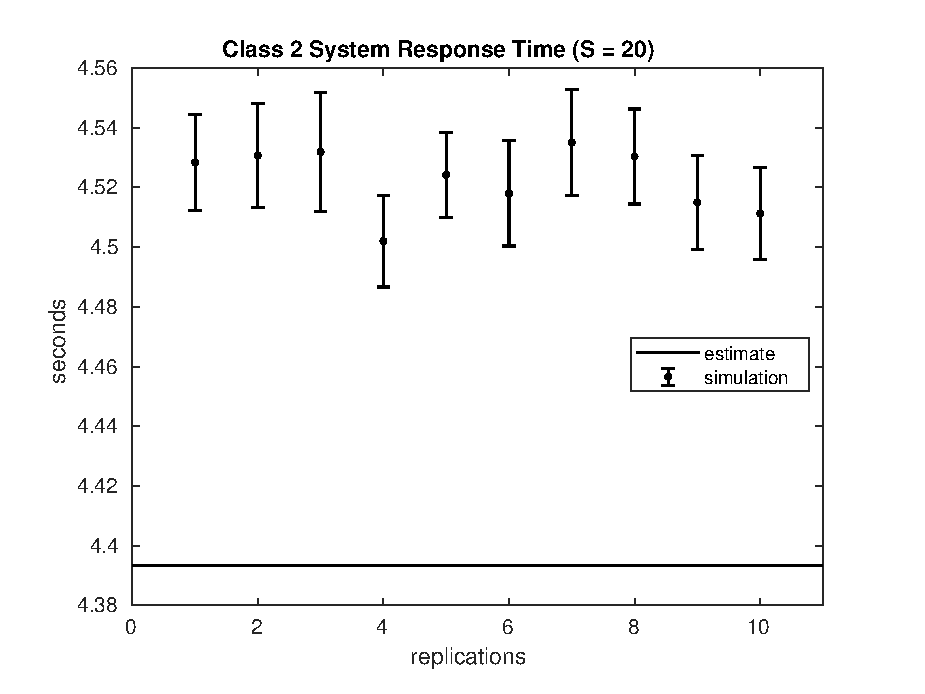
\includegraphics[width=\textwidth]{figures/simul/20_500K_s2}
\caption{$S = 20$}
\label{20_s2}
\end{subfigure}
%
\begin{subfigure}[t]{0.49\textwidth}
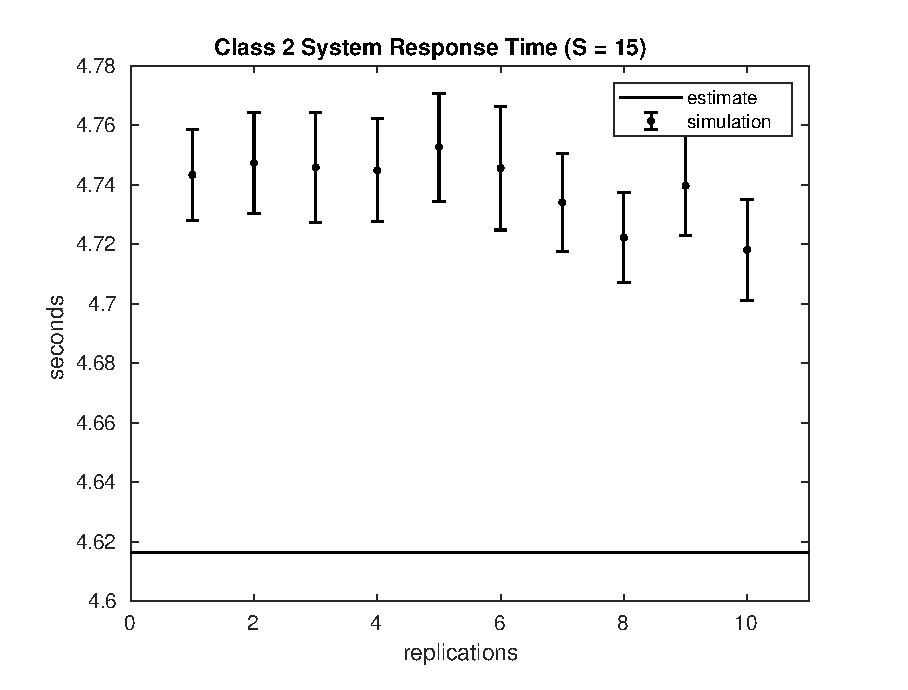
\includegraphics[width=\textwidth]{figures/simul/15_500K_s2}
\caption{$S = 15$}
\label{15_s2}
\end{subfigure}
%
\begin{subfigure}[t]{0.49\textwidth}
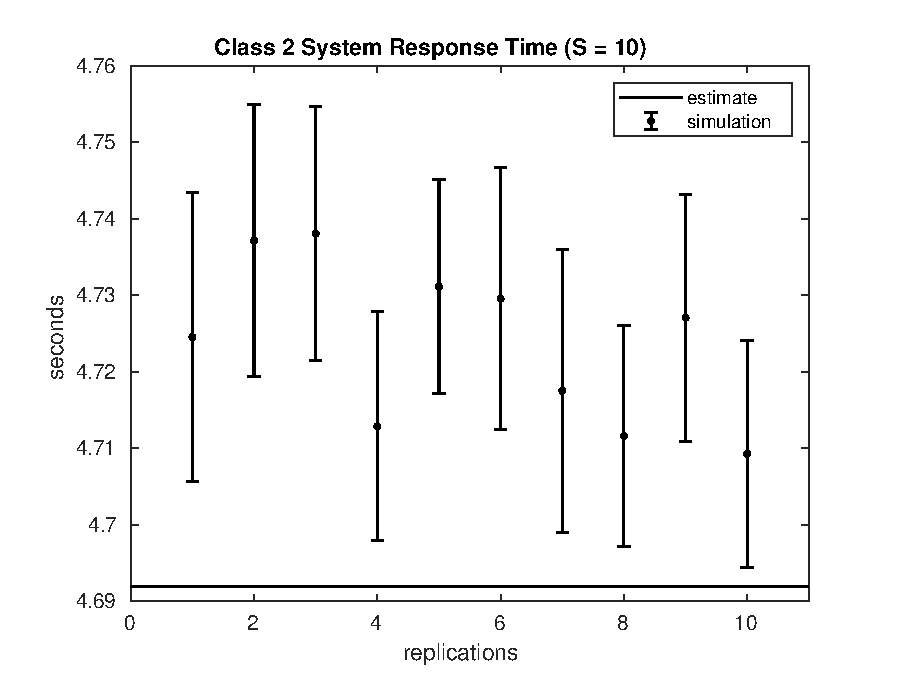
\includegraphics[width=\textwidth]{figures/simul/10_500K_s2}
\caption{$S = 10$}
\label{10_s2}
\end{subfigure}
%
\begin{subfigure}[t]{0.49\textwidth}
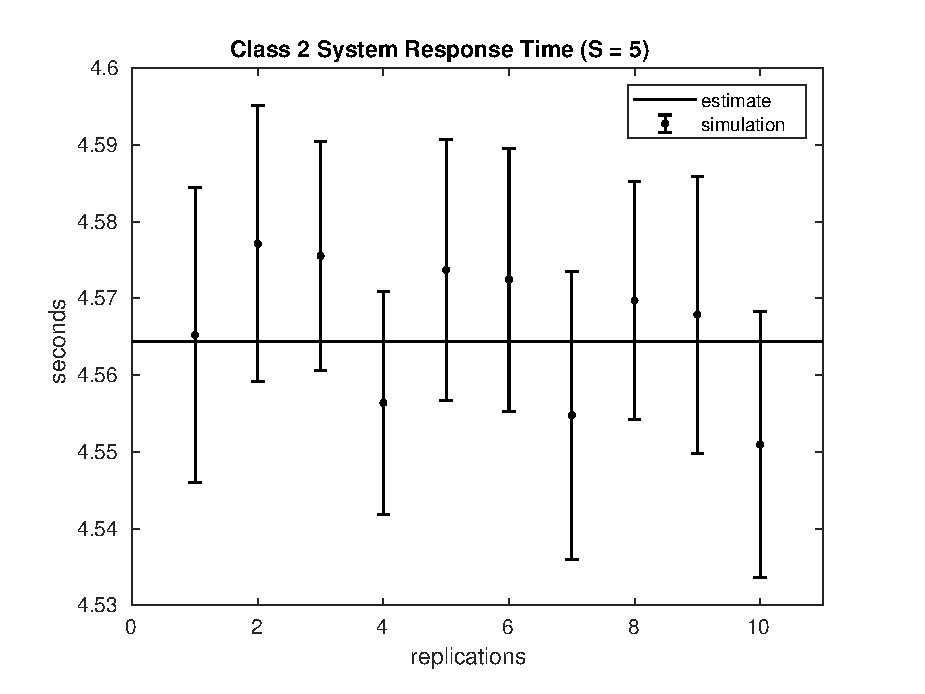
\includegraphics[width=\textwidth]{figures/simul/5_500K_s2}
\caption{$S = 5$}
\label{5_s2}
\end{subfigure}
%
\caption{tempo di risposta sistema classe 2}
\label{plot:s2}
\end{figure}
%
%
\begin{table}[!h]
\begin{adjustbox}{width=\textwidth}
\begin{tabular}{c|r@{.}l|r@{.}l|r@{.}l|r@{.}l}
& \multicolumn{2}{|c|}{$S=20$}
& \multicolumn{2}{|c|}{$S=15$} 
& \multicolumn{2}{|c|}{$S=10$} 
& \multicolumn{2}{|c}{$S=5$} 
\\          
\hline
R1      & $4$&$5284 \pm 0.0160$ & $4$&$7433 \pm 0.0154$ & $4$&$7245 \pm 0.0188$ & $4$&$5652 \pm 0.0192$ \\
R2      & $4$&$5307 \pm 0.0174$ & $4$&$7473 \pm 0.0170$ & $4$&$7371 \pm 0.0178$ & $4$&$5771 \pm 0.0180$ \\
R3      & $4$&$5319 \pm 0.0199$ & $4$&$7458 \pm 0.0185$ & $4$&$7381 \pm 0.0166$ & $4$&$5755 \pm 0.0149$ \\
R4      & $4$&$5020 \pm 0.0154$ & $4$&$7448 \pm 0.0173$ & $4$&$7129 \pm 0.0150$ & $4$&$5564 \pm 0.0145$ \\
R5      & $4$&$5242 \pm 0.0142$ & $4$&$7526 \pm 0.0181$ & $4$&$7311 \pm 0.0139$ & $4$&$5737 \pm 0.0170$ \\
R6      & $4$&$5180 \pm 0.0176$ & $4$&$7456 \pm 0.0208$ & $4$&$7295 \pm 0.0171$ & $4$&$5724 \pm 0.0171$ \\
R7      & $4$&$5351 \pm 0.0177$ & $4$&$7340 \pm 0.0164$ & $4$&$7175 \pm 0.0185$ & $4$&$5548 \pm 0.0187$ \\
R8      & $4$&$5303 \pm 0.0159$ & $4$&$7222 \pm 0.0151$ & $4$&$7116 \pm 0.0144$ & $4$&$5697 \pm 0.0155$ \\
R9      & $4$&$5150 \pm 0.0157$ & $4$&$7396 \pm 0.0168$ & $4$&$7271 \pm 0.0161$ & $4$&$5679 \pm 0.0180$ \\
R10     & $4$&$5113 \pm 0.0155$ & $4$&$7181 \pm 0.0170$ & $4$&$7093 \pm 0.0148$ & $4$&$5510 \pm 0.0173$ \\
EST     & $4$&$3935$            & $4$&$6165$            & $4$&$6920$            & $4$&$5644$            \\
\epsmx  & $0$&$1593 \ (3.5\%)$  & $0$&$1542 \ (3.2\%)$  & $0$&$0629 \ (1.3\%)$  & $0$&$0307 \ (0.7\%)$    
\end{tabular}
\end{adjustbox}
\caption{tempo di risposta sistema classe 2}
\label{tab:s2}
\end{table}

%%%%%%%%%%%%%%%%%%%%%%%%%%%%%%%%%%%%%%%%%%%%%%%%%%%%%%%%%%%%%%%%%%%%%%%%%%%%%%%%
\subsection{Tempo di Risposta Sistema}
Con l'aggiunta dei job di classe 1 nel calcolo del tempo di risposta globale del
sistema, la situazione non cambia, infatti, come mostrato in 
figura~\ref{plot:s} e tabella~\ref{tab:s}, si ottiene il minor tempo di risposta
nel caso in cui $S=20$, e anche in questo caso è evidente l'influenza della
percentuale di interruzione che induce alla sottostima, anche se con un errore
massimo più contenuto (al più del $2.7\%$), più precisa invece la stima
del caso $S=5$ (\epsmx$=0.5\%$).
\begin{figure}[!h]
\centering
%
\begin{subfigure}[t]{0.49\textwidth}
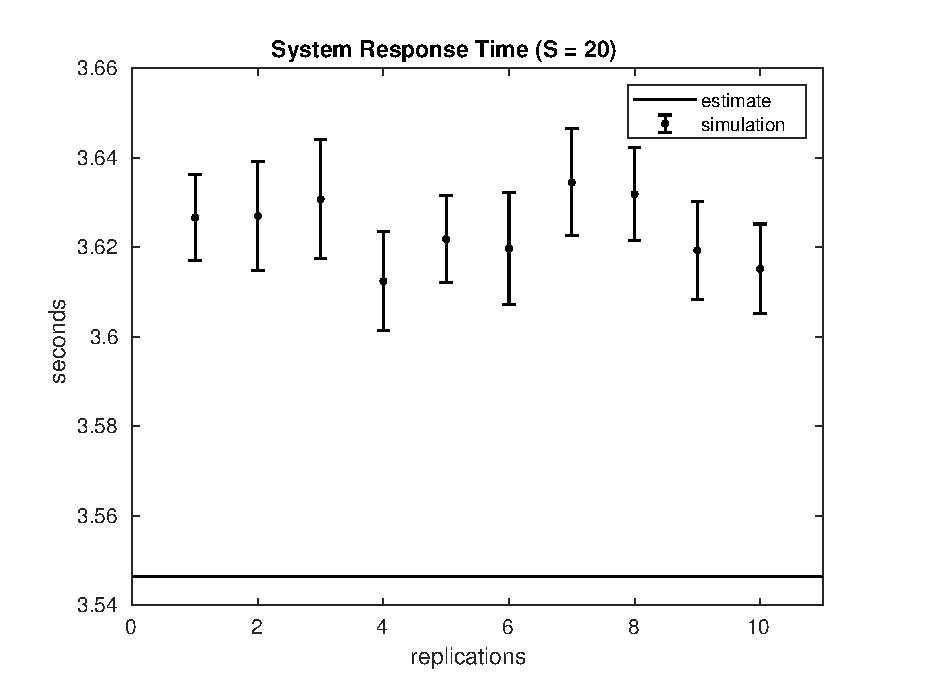
\includegraphics[width=\textwidth]{figures/simul/20_500K_s}
\caption{$S = 20$}
\label{20_s}
\end{subfigure}
%
\begin{subfigure}[t]{0.49\textwidth}
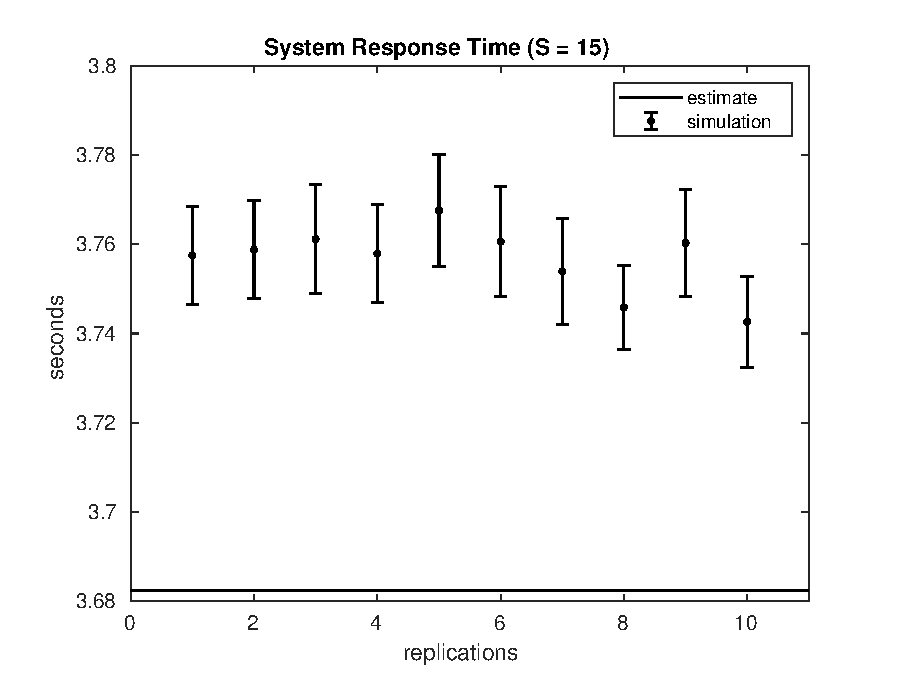
\includegraphics[width=\textwidth]{figures/simul/15_500K_s}
\caption{$S = 15$}
\label{15_s}
\end{subfigure}
%
\begin{subfigure}[t]{0.49\textwidth}
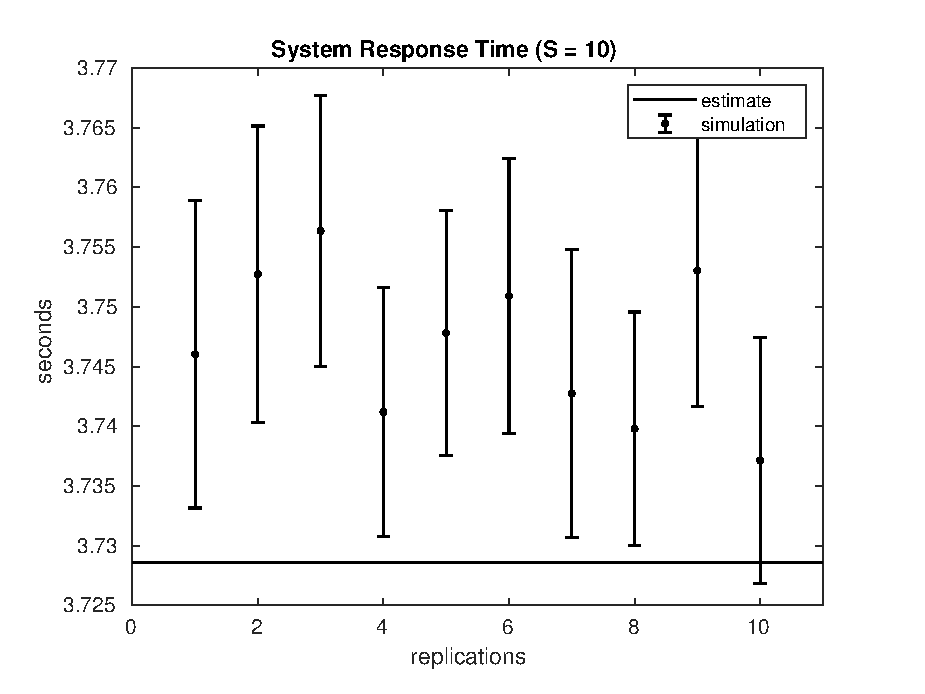
\includegraphics[width=\textwidth]{figures/simul/10_500K_s}
\caption{$S = 10$}
\label{10_s}
\end{subfigure}
%
\begin{subfigure}[t]{0.49\textwidth}
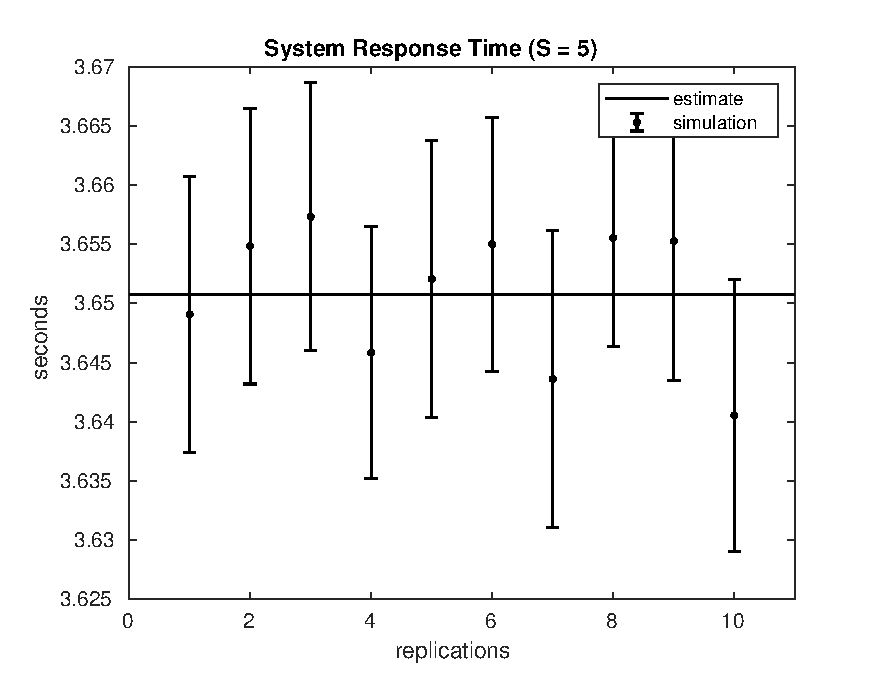
\includegraphics[width=\textwidth]{figures/simul/5_500K_s}
\caption{$S = 5$}
\label{5_s}
\end{subfigure}
%
\caption{tempo di risposta sistema}
\label{plot:s}
\end{figure}
%
%
\begin{table}[!h]
\begin{adjustbox}{width=\textwidth}
\begin{tabular}{c|r@{.}l|r@{.}l|r@{.}l|r@{.}l}
& \multicolumn{2}{|c|}{$S=20$}
& \multicolumn{2}{|c|}{$S=15$} 
& \multicolumn{2}{|c|}{$S=10$} 
& \multicolumn{2}{|c}{$S=5$} 
\\          
\hline
R1      & $3$&$6266 \pm 0.0096$ & $3$&$7575 \pm 0.0109$ & $3$&$7460 \pm 0.0129$ & $3$&$6491 \pm 0.0117$ \\
R2      & $3$&$6269 \pm 0.0121$ & $3$&$7588 \pm 0.0110$ & $3$&$7527 \pm 0.0124$ & $3$&$6548 \pm 0.0117$ \\
R3      & $3$&$6307 \pm 0.0133$ & $3$&$7611 \pm 0.0122$ & $3$&$7564 \pm 0.0114$ & $3$&$6573 \pm 0.0113$ \\
R4      & $3$&$6124 \pm 0.0110$ & $3$&$7579 \pm 0.0110$ & $3$&$7412 \pm 0.0105$ & $3$&$6458 \pm 0.0106$ \\
R5      & $3$&$6218 \pm 0.0097$ & $3$&$7675 \pm 0.0126$ & $3$&$7478 \pm 0.0103$ & $3$&$6521 \pm 0.0117$ \\
R6      & $3$&$6197 \pm 0.0125$ & $3$&$7606 \pm 0.0124$ & $3$&$7509 \pm 0.0115$ & $3$&$6550 \pm 0.0107$ \\
R7      & $3$&$6344 \pm 0.0119$ & $3$&$7539 \pm 0.0119$ & $3$&$7427 \pm 0.0120$ & $3$&$6436 \pm 0.0126$ \\
R8      & $3$&$6318 \pm 0.0103$ & $3$&$7459 \pm 0.0095$ & $3$&$7398 \pm 0.0098$ & $3$&$6555 \pm 0.0092$ \\
R9      & $3$&$6193 \pm 0.0109$ & $3$&$7603 \pm 0.0119$ & $3$&$7530 \pm 0.0114$ & $3$&$6553 \pm 0.0117$ \\
R10     & $3$&$6152 \pm 0.0100$ & $3$&$7426 \pm 0.0102$ & $3$&$7372 \pm 0.0103$ & $3$&$6406 \pm 0.0115$ \\
EST     & $3$&$5465$            & $3$&$6825$            & $3$&$7286$            & $3$&$6508$            \\
\epsmx  & $0$&$0999 \ (2.7\%)$  & $0$&$0976 \ (2.6\%)$  & $0$&$0392 \ (1.0\%)$  & $0$&$0179 \ (0.5\%)$    
\end{tabular}
\end{adjustbox}
\caption{tempo di risposta sistema}
\label{tab:s}
\end{table}

%%%%%%%%%%%%%%%%%%%%%%%%%%%%%%%%%%%%%%%%%%%%%%%%%%%%%%%%%%%%%%%%%%%%%%%%%%%%%%%%
%%%%%%%%%%%%%%%%%%%%%%%%%%%%%%%%%%%%%%%%%%%%%%%%%%%%%%%%%%%%%%%%%%%%%%%%%%%%%%%%
%%%%%%%%%%%%%%%%%%%%%%%%%%%%%%%%%%%%%%%%%%%%%%%%%%%%%%%%%%%%%%%%%%%%%%%%%%%%%%%%
%%%%%%%%%%%%%%%%%%%%%%%%%%%%%%%%%%%%%%%%%%%%%%%%%%%%%%%%%%%%%%%%%%%%%%%%%%%%%%%%
%%%%%%%%%%%%%%%%%%%%%%%%%%%%%%%%%%%%%%%%%%%%%%%%%%%%%%%%%%%%%%%%%%%%%%%%%%%%%%%%
